\documentclass[12pt,]{book}
%\usepackage{xcolor}
\usepackage{lmodern}
\usepackage{setspace}
\setstretch{1}
\usepackage{amssymb,amsmath}
\usepackage{ifxetex,ifluatex}
\usepackage{fixltx2e} % provides \textsubscript
\ifnum 0\ifxetex 1\fi\ifluatex 1\fi=0 % if pdftex
  \usepackage[T1]{fontenc}
  \usepackage[utf8]{inputenc}
\else % if luatex or xelatex
  \ifxetex
    \usepackage{mathspec}
  \else
    \usepackage{fontspec}
  \fi
  \defaultfontfeatures{Ligatures=TeX,Scale=MatchLowercase}
    \setmainfont[]{Montserrat}
\fi
% use upquote if available, for straight quotes in verbatim environments
\IfFileExists{upquote.sty}{\usepackage{upquote}}{}
% use microtype if available
\IfFileExists{microtype.sty}{%
\usepackage{microtype}
\UseMicrotypeSet[protrusion]{basicmath} % disable protrusion for tt fonts
}{}
\usepackage[marginpar=2cm, top=3cm, bottom=4cm]{geometry}
\usepackage{hyperref}
\PassOptionsToPackage{usenames,dvipsnames}{xcolor} % color is loaded by hyperref
\hypersetup{unicode=true,
            colorlinks=true,
            citecolor=teal,
            linkcolor=lime,
            urlcolor=blue,
            breaklinks=true}
\urlstyle{same}  % don't use monospace font for urls
\usepackage[numbers]{natbib}
\bibliographystyle{plainnat}
\usepackage{color}
\usepackage{fancyvrb}
\newcommand{\VerbBar}{|}
\newcommand{\VERB}{\Verb[commandchars=\\\{\}]}
\DefineVerbatimEnvironment{Highlighting}{Verbatim}{commandchars=\\\{\}}
% Add ',fontsize=\small' for more characters per line
\usepackage{framed}
\definecolor{shadecolor}{RGB}{248,248,248}
\newenvironment{Shaded}{\begin{snugshade}}{\end{snugshade}}
\newcommand{\KeywordTok}[1]{\textcolor[rgb]{0.13,0.29,0.53}{\textbf{#1}}}
\newcommand{\DataTypeTok}[1]{\textcolor[rgb]{0.13,0.29,0.53}{#1}}
\newcommand{\DecValTok}[1]{\textcolor[rgb]{0.00,0.00,0.81}{#1}}
\newcommand{\BaseNTok}[1]{\textcolor[rgb]{0.00,0.00,0.81}{#1}}
\newcommand{\FloatTok}[1]{\textcolor[rgb]{0.00,0.00,0.81}{#1}}
\newcommand{\ConstantTok}[1]{\textcolor[rgb]{0.00,0.00,0.00}{#1}}
\newcommand{\CharTok}[1]{\textcolor[rgb]{0.31,0.60,0.02}{#1}}
\newcommand{\SpecialCharTok}[1]{\textcolor[rgb]{0.00,0.00,0.00}{#1}}
\newcommand{\StringTok}[1]{\textcolor[rgb]{0.31,0.60,0.02}{#1}}
\newcommand{\VerbatimStringTok}[1]{\textcolor[rgb]{0.31,0.60,0.02}{#1}}
\newcommand{\SpecialStringTok}[1]{\textcolor[rgb]{0.31,0.60,0.02}{#1}}
\newcommand{\ImportTok}[1]{#1}
\newcommand{\CommentTok}[1]{\textcolor[rgb]{0.56,0.35,0.01}{\textit{#1}}}
\newcommand{\DocumentationTok}[1]{\textcolor[rgb]{0.56,0.35,0.01}{\textbf{\textit{#1}}}}
\newcommand{\AnnotationTok}[1]{\textcolor[rgb]{0.56,0.35,0.01}{\textbf{\textit{#1}}}}
\newcommand{\CommentVarTok}[1]{\textcolor[rgb]{0.56,0.35,0.01}{\textbf{\textit{#1}}}}
\newcommand{\OtherTok}[1]{\textcolor[rgb]{0.56,0.35,0.01}{#1}}
\newcommand{\FunctionTok}[1]{\textcolor[rgb]{0.00,0.00,0.00}{#1}}
\newcommand{\VariableTok}[1]{\textcolor[rgb]{0.00,0.00,0.00}{#1}}
\newcommand{\ControlFlowTok}[1]{\textcolor[rgb]{0.13,0.29,0.53}{\textbf{#1}}}
\newcommand{\OperatorTok}[1]{\textcolor[rgb]{0.81,0.36,0.00}{\textbf{#1}}}
\newcommand{\BuiltInTok}[1]{#1}
\newcommand{\ExtensionTok}[1]{#1}
\newcommand{\PreprocessorTok}[1]{\textcolor[rgb]{0.56,0.35,0.01}{\textit{#1}}}
\newcommand{\AttributeTok}[1]{\textcolor[rgb]{0.77,0.63,0.00}{#1}}
\newcommand{\RegionMarkerTok}[1]{#1}
\newcommand{\InformationTok}[1]{\textcolor[rgb]{0.56,0.35,0.01}{\textbf{\textit{#1}}}}
\newcommand{\WarningTok}[1]{\textcolor[rgb]{0.56,0.35,0.01}{\textbf{\textit{#1}}}}
\newcommand{\AlertTok}[1]{\textcolor[rgb]{0.94,0.16,0.16}{#1}}
\newcommand{\ErrorTok}[1]{\textcolor[rgb]{0.64,0.00,0.00}{\textbf{#1}}}
\newcommand{\NormalTok}[1]{#1}
\usepackage{longtable,booktabs}
\usepackage{graphicx,grffile}
\makeatletter
\def\maxwidth{\ifdim\Gin@nat@width>\linewidth\linewidth\else\Gin@nat@width\fi}
\def\maxheight{\ifdim\Gin@nat@height>\textheight\textheight\else\Gin@nat@height\fi}
\makeatother
% Scale images if necessary, so that they will not overflow the page
% margins by default, and it is still possible to overwrite the defaults
% using explicit options in \includegraphics[width, height, ...]{}
\setkeys{Gin}{width=\maxwidth,height=\maxheight,keepaspectratio}
\IfFileExists{parskip.sty}{%
\usepackage{parskip}
}{% else
\setlength{\parindent}{0pt}
\setlength{\parskip}{6pt plus 2pt minus 1pt}
}
\setlength{\emergencystretch}{3em}  % prevent overfull lines
\providecommand{\tightlist}{%
  \setlength{\itemsep}{0pt}\setlength{\parskip}{0pt}}
\setcounter{secnumdepth}{5}
% Redefines (sub)paragraphs to behave more like sections
\ifx\paragraph\undefined\else
\let\oldparagraph\paragraph
\renewcommand{\paragraph}[1]{\oldparagraph{#1}\mbox{}}
\fi
\ifx\subparagraph\undefined\else
\let\oldsubparagraph\subparagraph
\renewcommand{\subparagraph}[1]{\oldsubparagraph{#1}\mbox{}}
\fi

%%% Use protect on footnotes to avoid problems with footnotes in titles
\let\rmarkdownfootnote\footnote%
\def\footnote{\protect\rmarkdownfootnote}

%%% Change title format to be more compact
\usepackage{titling}

% Create subtitle command for use in maketitle
\newcommand{\subtitle}[1]{
  \posttitle{
    \begin{center}\large#1\end{center}
    }
}

\setlength{\droptitle}{-2em}
  \title{}
  \pretitle{\vspace{\droptitle}}
  \posttitle{}
  \author{}
  \preauthor{}\postauthor{}
  \date{}
  \predate{}\postdate{}

% Améliore l'esthétique de la police
\usepackage{lmodern}
%Packages pour créer des tableaux 
\usepackage{longtable} % Pour des tableaux dont la longueur dépasse une feuille A4
\usepackage{tabularx} % Pour des tableaux à largeur définie
\usepackage{array} % Pour améliorer la qualité typographique des tableaux.
\usepackage{siunitx}
\usepackage[font=small,labelfont=bf]{caption}

%%%%%
\usepackage{booktabs}
\usepackage{longtable}
\usepackage{array}
\usepackage{multirow}
\usepackage{wrapfig}
\usepackage{float}
\usepackage{colortbl}
\usepackage{pdflscape}
\usepackage{tabu}
\usepackage{threeparttable}
\usepackage{booktabs}
\usepackage{longtable}
\usepackage{array}
\usepackage{multirow}
\usepackage[table]{xcolor}
\usepackage{wrapfig}
\usepackage{float}
\usepackage{colortbl}
\usepackage{pdflscape}
\usepackage{tabu}
\usepackage{threeparttable}
\usepackage{threeparttablex}
\usepackage[normalem]{ulem}
\usepackage{makecell}
\usepackage{pdfpages}
\usepackage{amsthm}
\newtheorem{theorem}{Theorem}[chapter]
\newtheorem{lemma}{Lemma}[chapter]
\theoremstyle{definition}
\newtheorem{definition}{Definition}[chapter]
\newtheorem{corollary}{Corollary}[chapter]
\newtheorem{proposition}{Proposition}[chapter]
\theoremstyle{definition}
\newtheorem{example}{Example}[chapter]
\theoremstyle{definition}
\newtheorem{exercise}{Exercise}[chapter]
\theoremstyle{remark}
\newtheorem*{remark}{Remark}
\newtheorem*{solution}{Solution}
\begin{document}

%Page de garde
\begin{titlepage}
\frontmatter
\begin{figure}[t]

\includegraphics[width=5cm]{figures-ext/LogoParisDescartes}
\end{figure}
\begin{center}
UNIVERSITÉ PARIS DESCARTES \\
\vspace*{1cm}
\textbf{ED 474 Frontières du vivant}\\
\vspace*{0,5cm}
\textit{Institut Curie, PSL Research University, Mines Paris Tech, Inserm U900 \\Paris, France}\\
\vspace*{1cm}
\LARGE{\textbf{UNSUPERVISED DECONVOLUTION OF CELL AND ENVIRONMENT SPECIFIC SIGNALS AND
THEIR INTERACTIONS FROM COMPLEX MIXTURES IN BIOLOGICAL SAMPLES}}\\
\large{\textbf{Par Urszula Czerwińska}}\\
\vspace*{1cm}
Thèse de doctorat de Biostatistique\\
\vspace*{1cm}
Thèse dirigée par Andrei Zinovyev et Vassili Soumelis\\
\vspace*{1cm}
\small{Présentée et soutenue publiquement le 2 octobre 2018}\\
\end{center}
\vspace*{1cm}
\begin{footnotesize}
Devant un jury composé de : \\
\begin{tabular}{lll}
Andrei Zinovyev & directeur de thèse - PSL\\
Vassili Soumelis & directeur de thèse - PSL\\
Prénom NOM & [fonction] - université\\

\end{tabular}
\end{footnotesize}

\begin{figure}[b]
\begin{center}

\includegraphics{figures-ext/creativecommons}
\end{center}
\end{figure}




\clearpage


%Abstract
\newpage
\thispagestyle{empty}
\noindent % Supprime le retrait de paragraphe

\textbf{Title: }
Déconvolution non supervisée de signaux spécifiques aux cellules dans leur environnement et leurs interactions à partir de mélanges complexes dans des échantillons biologiques
\vskip 1cm
\textbf{Résumé (français) :}
\vskip 1cm
\noindent
\textbf{Title: }
Unsupervised deconvolution of cell and environment specific signals and their interactions from complex mixtures in biological samples
\vskip 1cm
\noindent
\textbf{Abstract:}
In many fields of science (biology, technology, sociology) observations on a studied system represent complex mixtures of signals of various origin. Tumors are engulfed in a complex microenvironment (TME) that critically impacts progression and response to therapy. It includes tumor cells, fibroblasts, and a diversity of immune cells. Most studies have focused on individual cell types in model tumor systems, and/or on individual molecules mediating a crosstalk between two cells. Unraveling the complexity, organization, and mutual interactions of TME cellular components represents a major challenge.
Methods for deconvolution of complex mixtures of signals have been developed in signal processing field. It is known that under some assumptions, it is possible to separate complex signal mixtures, using classical and advanced methods of source separation and dimension reduction. Our recent large-scale analysis of more than 6500 tumor transcriptomes, applying classical blind source separation methods showed that we can reliably separate signals coming from tumor microenvironment from the tumor-specific signals and various technical artifacts. However, the precise composition of the immune-related signals in a tumor sample remains to be deciphered.

In this project, we develop and apply the advanced methodology of signal deconvolution to decipher sources of signals shaping transcriptomes of tumor samples, with a particular focus on immune-related signals. So far, we managed to deconvolute successfully immune-related signal into groups related to immune cell-types in six breast cancer datasets. However, the precise composition of the immune-related signals and their interactions in a tumor sample remains to be deciphered and our method needs to be calibrated.

We are going to release our processing pipeline in a form of an R package. This will allow the scientific community profit from our analytical pipeline and easily reproduce our results.

In the case of success of this project, the results will be helpful in the detemining diagnosis and treatment of cancer, especially for immunotherapies.
\vskip 1cm
\noindent
\textbf{Mots-clés (français) :} microenvironnement tumoral, biologie des systèmes de cancer, analyse de données transcriptomiques, analyse de données monocellulaires, bioinformatique, hétérogénéité,  séparation aveugle de source, apprentissage non supervisé, cancer, oncologie, immunologie
\vskip 1cm
\noindent
\textbf{Keywords:} tumor microenvironment, cancer systems biology, transcriptome data analysis, single cell data analysis, bioinformatics, heterogeneity, blind sources separation, unsupervised learning, cancer, oncology, immunology


%Dédicace
\newpage
\emph{Dédicace}
\vspace*{\fill}

 \begin{quote}
\emph{\textbf{And now, let's repeat the Non-Conformist Oath!\\
I promise to be different!\\
I promise to be unique!\\
I promise not to repeat things other people say!}}\\
— Steve Martin, \textit{A Wild and Crazy Guy (1978)}\\
 \end{quote}
 \vspace*{\fill}


%Remerciements
\newpage
\thispagestyle{empty}
\begin{center}
\large{\textbf{Avertissement}}
\end{center}
\vspace{2cm}
Cette thèse de doctorat est le fruit d’un travail approuvé par le jury de soutenance et
réalisé dans le but d’obtenir le diplôme d’Etat de docteur de philosophie. Ce document
est mis à disposition de l’ensemble de la communauté universitaire élargie.
Il est soumis à la propriété intellectuelle de l’auteur. Ceci implique une obligation de
citation et de référencement lors de l’utilisation de ce document.
D’autre part, toute contrefaçon, plagiat, reproduction illicite encourt toute poursuite
pénale.
\vspace*{\fill}

\emph{Code de la Propriété Intellectuelle. Articles L 122.4 \newline
Code de la Propriété Intellectuelle. Articles L 335.2-L 335.10}


\newpage
\thispagestyle{empty}
\begin{center}
%\large{\textbf{Remerciments}}
\large{\textbf{Remerciments}}
\end{center}
\vspace{2cm}
Merci tout le monde

\end{titlepage}


{
\hypersetup{linkcolor=black}
\setcounter{tocdepth}{4}
\tableofcontents
}
\hypersetup{linkcolor=black}
\listoftables

\hypersetup{linkcolor=black}
\listoffigures
\hypertarget{preamble-about-interdisciplinary-research}{%
\chapter*{Preamble about Interdisciplinary
Research}\label{preamble-about-interdisciplinary-research}}
\addcontentsline{toc}{chapter}{Preamble about Interdisciplinary
Research}

\setcounter{page}{15}\renewcommand{\thepage}{\arabic{page}}

\begin{quote}
\emph{We are not students of some subject matter, but students of
problems. And problems may cut right across the borders of any subject
matter or discipline.} --- Karl Popper
\end{quote}

The piece of work you have between your hands or on your screen should
collect fruits of an interdisciplinary research, or at least, was
conceived in an interdisciplinary environment of Center for
Interdisciplinary Research in Paris (CRI) in École doctorale
\emph{Frontières du Vivant} (FdV) . CRI's main mission can be formulated
as follows:

\begin{quote}
\emph{to empower the students to take initiative and develop their own
research projects \textbf{at the crossroads of life, learning, and
digital sciences}.} \citep{CRIweb}
\end{quote}

Interdisciplinarity has many definitions and meanings. According to the
book \emph{Facilitating Interdisciplinary Research} \citep{FIRbook}

\begin{quote}
\emph{Interdisciplinary research and education are inspired by the drive
to solve \textbf{complex questions} and problems, whether generated by
scientific curiosity or by society, and lead researchers in different
disciplines to meet at the \textbf{interfaces} and \textbf{frontiers} of
those disciplines and even to \textbf{cross frontiers} to \textbf{form
new disciplines}.}
\end{quote}

For me, the essence of interdisciplinarity is the need to solve a
complex problem, whatever expertise would be necessary to solve it. I
consider that fighting cancer disease, deciphering cancer heterogeneity
and its interactions with immune systems is a cause worth an
interdisciplinary effort. This is even more true in the era of big data
that demand quantitative tools in order to extract information and
knowledge.

Though this preamble I would like not only praise the interdisciplinary
research but also underline possible limitations and constraints that
come with it and which could affect this thesis.

\hypertarget{what-does-interdisciplinarity-in-science-mean-in-xxi-century}{%
\section*{What does interdisciplinarity in science mean in XXI
century?}\label{what-does-interdisciplinarity-in-science-mean-in-xxi-century}}
\addcontentsline{toc}{section}{What does interdisciplinarity in science
mean in XXI century?}

In the ancient history, being formed and practice multiple disciplines
was not anything unusual which is strongly reflected in Greek philosophy
initiating the dispute about the division and hierarchical
classification of knowledge. \citep{Slavicek2012}. Figures as Aristotle
and Leonardo Da Vinci, that can be called \emph{homo universals} served
different disciplines from arts through history, natural sciences to
mathematics. With time human knowledge about the word, i.e.~natural
sciences got bigger and bigger, to the point that it became hard to
master all the disciplines. The specialisation would allow to study in
deep a certain subject and make discoveries about it. And even if,
interdisciplinary efforts never stopped, for long time they were not
mainstream in scientific communities divided into academies, chairs and
specialization.

How we can define these separate units? Different fields differ in term
of concept, method, tools, processes and theories \citep{Slavicek2012}.
Thanks to division into scientific disciplines certain order is
conserved across space and time. Hierarchical classification of
knowledge comes with human nature.

However, specialisation came with a price,

\begin{quote}
\emph{advancing specialisation leads to gaps in the level of
comprehension between individual disciplines and eventually gives rise
to the demand for interdisciplinarity - in order to close the gaps
between disciplines.}\citep{Slavicek2012}
\end{quote}

Nowadays, the knowledge is accessible and popular, therefore we can
profit from achievements of different disciplines thanks to easy mean of
communication. Two different terms can be defined to initiatives that
use the knowledge of different specialities: multidisciplinarity which
is a sum of efforts of different disciplines and interdisciplinarity
that allows to profit from synergy of multiple disciplines (Fig.
\ref{fig:multidisc}). With interdisciplinary research and education come
flexibility, creativity and novelty but also limit of depth on ingested
knowledge and possibilities of cross-interactions between disciplines.

\begin{figure}

{\centering 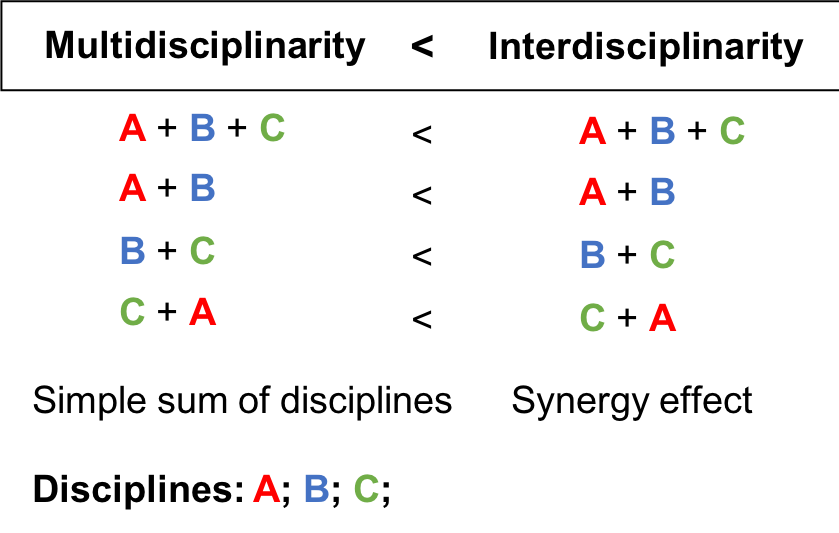
\includegraphics[width=1\linewidth]{figures-ext/multidisc} 

}

\caption{\textbf{Symbolic illustration of sum
(multidisciplinarity) versus synergy (interdisciplinarity)}, an
interdisciplinary project should have an added value compared to a
multidisciplinary one. Inspired from \citep{Slavicek2012}.}\label{fig:multidisc}
\end{figure}






\emph{What does it mean to be truly interdisciplinary in science today
and why disciplines still exist? Do they?}

\begin{quote}
\emph{Scientists tend to resist interdisciplinary inquiries into their
own territory. In many instances, such parochialism is founded on the
fear that intrusion from other disciplines would compete unfairly for
limited financial resources and thus diminish their own opportunity for
research} ---
\href{http://www.azquotes.com/author/28130-Hannes_Alfven}{Hannes Alfvén}
\end{quote}

An example of truly interdisciplinary research can be work on the string
theory that makes advance both mathematics and theoretical physics. Also
new disciplines that recently emerged as biophysics and bioinformatics
are fuit of the interdisciplinary approach.

Bioinformatics and/or computational biology is an interesting case.
Working in this field being between biology, medecine, computer science,
mathematics and statistics, the role of a computational biologist is
sometimes reduced to a service. A biological lab may need a
computational biologist to perform an analysis, restructure the data,
that is needed for the biological discovery. Often, there is not enough
space for research in computational biology itself, where the discovery
does not depend on the original data but on tools and approaches to
complex, data-intensive biological problems. It may happed also the
other way round, when a computational biologist ask a bench researcher
to perform an experiment only to prove a theory. In both cases, the
long-term interdisciplinary partnership would probably fail. A wet and
dry researches should collaborate as equal with important research
advances on both side to assure a long term equilibrium.

Crossing frontiers is not an easy task, and it was even more difficult
in its beginnings. Some examples of early interdisciplinary efforts are
nicely described by Ledford et al. \citep{Ledford2015} in \emph{Nature}
special issue on
\href{https://www.nature.com/news/interdisciplinarity-1.18295}{Interdisciplinarity}.
It illustrates Theodore Brown in 1980s, while trying to organise a new
interdisciplinary research project and reorganise university space to
engage exchange between students of different faculties, he encounter a
lot of reluctance.

\begin{quote}
\emph{And then there was the stigma. ``Interdisciplinary research is for
people who aren't good enough to make it in their own field,'' an
illustrious physicist chided} \citep{Ledford2015}.
\end{quote}

The story seems to end up with a happy ending of 40-milion US dollars
grant and foundation of Beckman Institute for Advanced Science and
Technology. However, recruiting open-minded director to lead this
unconventional organisation was a struggle. Soon, the organisation
became a model for others and met a great scientific success (creation
of one of the first graphical web browsers).

Even though, since then the idea of interdisciplinary research spread
around the world. Still, not all problem got overcome.

\begin{quote}
\emph{``There's a huge push to call your work interdisciplinary,'' says
David Wood, a bioengineer at the University of Minnesota in Minneapolis.
``But there's still resistance to doing actual interdisciplinary
science''.}
\end{quote}

First, the institutions, universities where research is performed should
equip scientist with a passport to other disciplines, facilitate
exchange, funding the interdisciplinary research, accepting fusion of
disciplines as new ones. Then, a proper communication between
disciplines is necessary. Finally, forming interdisciplinary researches
is extremely challenging as it often requires extra effort from an
apprentice.

\emph{Are all the disciplines idependent units nowadays?}

Can we do molecular biology without technical, mathematical and
computational support? Can we study cognitive science without knowledge
of biology, physics and psychology? Can we advance medecine without
basic research in biology, physiology, electronics?

\emph{How interdisciplinarity changed over years? Are all disciplines
affected equally?}

From the chart (Fig. \ref{fig:interdisciplinary}) we can see that Social
Studies of Medicine seems to be the most interdisciplinary field. In
general Biology, Health and Biomedical Sciences seem to be more open
into flow of knowledge from other fields than humanities. On the extreme
opposite of health, Clinical Medecine appears to be very conservative
field.

\begin{figure}

{\centering 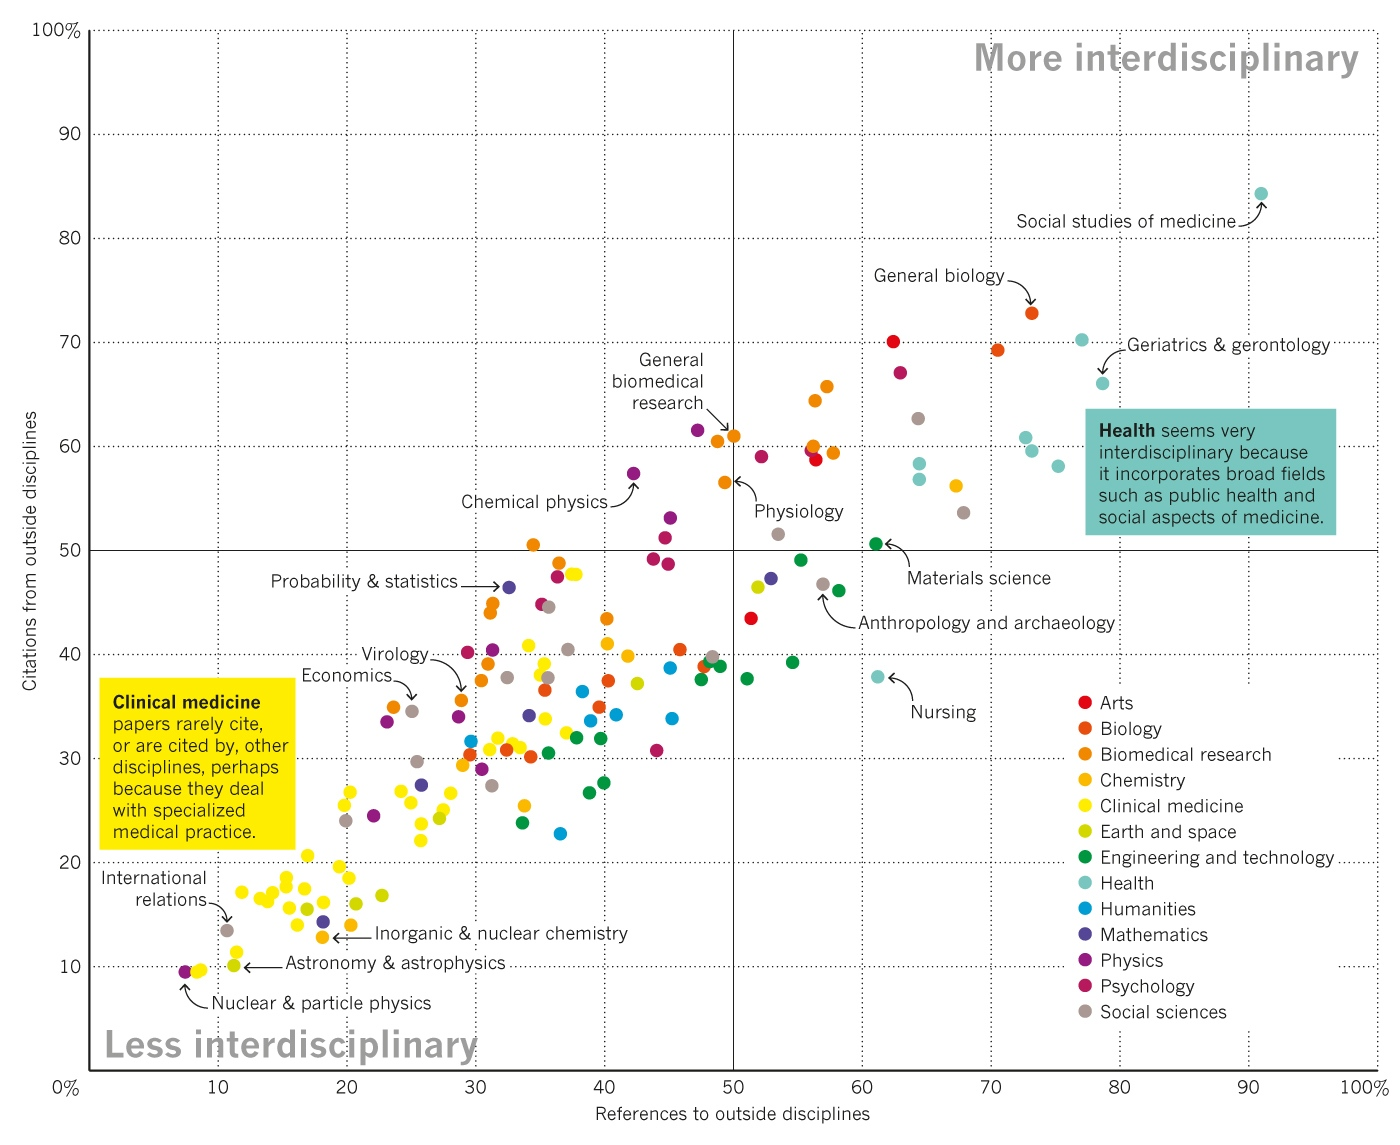
\includegraphics{figures-ext/interdisciplinary} 

}

\caption{\textbf{Interdisciplnarity of different
fields.} ``From 1950-2014, a field's position is determined by how much
its papers cite outside disciplines (x-axis), and by how much outside
disciplines subsequently cite its papers (y-axis). (Some years, certain
fields have too few references to be plotted.)''. Reprinted by
permission from Springer Nature \citep{VanNoorden2015} © 2015 Nature
America, Inc.~All rights reserved.}\label{fig:interdisciplinary}
\end{figure}









\hypertarget{strengths-weaknesses-opportunities-threats-swot-of-an-interdisciplinary-phd---personal-perspective}{%
\section*{Strengths, Weaknesses Opportunities, Threats (SWOT) of an
interdisciplinary PhD - personal
perspective}\label{strengths-weaknesses-opportunities-threats-swot-of-an-interdisciplinary-phd---personal-perspective}}
\addcontentsline{toc}{section}{Strengths, Weaknesses Opportunities,
Threats (SWOT) of an interdisciplinary PhD - personal perspective}

\begin{quote}
I'm not good enough to do well something I dislike. In fact, I find it
hard enough to do well something that I like --- Jim Watson, Succeeding
In Science: Some Rules Of Thumb
\end{quote}

Being formed first in double major in biology and mathematics, then
participating in interdisciplinary research projects during my master
studies, I can witness that learning curve of multiple disciples can be
steep. It is also often associated with frustration of not going deep
enough in all of disciplines or the feeling of being overwhelmed by the
amount of knowledge.

Coming with expertise of biology and mathematics, I got fascinated by
complex biological systems. One way of study high-dimensional data and
reduce them to smaller interpretable units. This is what I tempted to
achieve in this thesis in order to enrich our knowledge about tumor
microenvironment and possible contribute to orienting future research on
immunotherapies.

However, being an interdisciplinary researcher was not a privilege.
\emph{To which category do I belong?} \emph{To whom should I present my
work?} I often asked myself these questions. I also often encountered
lack of understanding where my methodological results were not bringing
enough of \emph{biological insights}. Or the constraints of my
biological application seemed very obscured and complicated for
mathematicians and my work often lacked \emph{important methodological
advances}.

\emph{Does it mean that my work is not accurate, useless?} Probably, for
many, it is not enough. However, I still hope that for some it is. I
enjoy working with data and statistics that serve an actual purpose. The
Tab. \ref{tab:SWOT} summarizes Strengths, Weaknesses, Opportunities and
Threats (SWOT analysis) of an interdisciplinary projects, in the way I
see it.

\rowcolors{2}{gray!6}{white}\begin{table}

\caption{\label{tab:SWOT}\textbf{SWOT analysis of Interdisciplinary research}}
\centering
\begin{tabular}[t]{|>{\centering\arraybackslash}p{9em}|>{\centering\arraybackslash}p{9em}|>{\centering\arraybackslash}p{9em}|>{\centering\arraybackslash}p{9em}|}
\hiderowcolors
\toprule
\rowcolor{Gray}  \textcolor{white}{\textbf{Strengths (internal, positive)}} & \textcolor{white}{\textbf{Weaknesses (internal, negative)}} & \textcolor{white}{\textbf{Opportunities (external, positive)}} & \textcolor{white}{\textbf{Threats (external, negative)}}\\
\midrule
\showrowcolors
Having a holistic view of the problem & Not seeing details of the problem & Mulitple possibilities to convey research & Spending too much time filling knowledge gap\\
Being supervised by multiple experts & Being in the missgle of a conflict of two experts & Take advantage of synergistic effect of fields & Inhibiting effect of oppinions from different fields\\
Joining expertises of different fields & Not covering in details all the disciplines & Doing a new discovery & Obtaining too generic results\\
Using new/non standart approach & Experiencing steep learning curve & Raising interest in different expert domains & Not mastering the specific vocabulary of different fields\\
Having better understanding of complex processes & Being in constant need of help of domain experts & Making progress & Not being understood\\
\addlinespace
Higher creativity &  & Creating a new field & Being hard to classify/ fall into a category\\
Having great flexibility &  & Sovling many problems impossible to solve with traditional approach & Being considered as superficial\\
Feeling a thrill of adventure &  &  & \\
Being open &  &  & \\
\bottomrule
\end{tabular}
\end{table}\rowcolors{2}{white}{white}



Besides conducting research that crosses the boundaries of one
discipline, I also could meet and work with inspiring people coping like
me with filling the gap in understanding of an interdisciplinary work,
multiple supervisors and reporting to many institutions. I gained (even
if only superficial) understanding of many topics in mathematics,
statistics, data science, immunology, cancer but also oral and written
presentation skills, time and work management

Is my thesis really interdisciplinary? Does biology profits from
mathematics and mathematics from biology? I will let you judge it.

What impact had biology on the statistical/mathematical modelling ? The
practical problems, systems that go beyond theoretical formulations
challenge the theoretical tools. In my work, I did my best to fuse
theory and practice that should serve a biological application. I can
image the project more complete if the results of my work would inspire
changes in biological experiments, uncover new paths to follow for
experimental biologists or translational researchers.

\hypertarget{general-context-of-the-thesis}{%
\section*{General context of the
thesis}\label{general-context-of-the-thesis}}
\addcontentsline{toc}{section}{General context of the thesis}

\begin{quote}
\emph{The universe will lead me where I need to go. I am like a leaf in
the stream of creation} --- Dirk Gently, Holistic detective
\end{quote}

When finishing my master I was looking for an interdisciplinary subject
where I could deepen my quantitative skills and apply to a real-life
healthcare problem. I came across a project proposed by Andrei Zinovyev
in close collaboration with Vassili Soumelis. I was quite anxious that
my knowledge of cancer immunology would not be sufficient to lead the
project to a success. I recognise that the complexity and heterogeneity
of immune systems are quite a mystery to me and even though I did my
best efforts to learn during these three years, I am still far for being
confortable.

The project started by causal exploration of different blind source
separation or dimension reduction techniques and their ability to
dissect bulk transcriptomic data into cell type-related units. We also
faced an important problem of lack of gold standard data that would
define efficiency and accuracy of different methods. I have spent void
efforts working of sophisticated simulation framework, I touched the
border of my capacities to solve important statistical issue. In the
meantime, many tools dissecting tumor bulk transcriptome were published.
Serving a similar purpose, they used different means and assumptions,
which leaved space for my project to continue. In my third year, I am
finally publishing a tool that performs the analysis I developed
together with the Sysbio team members, and I can apply it to a body of
publicly available data sets to learn about actual problem: the immune
system infiltrating cancers and the interactions occurring in the
environment (see \protect\hyperlink{deconica}{Chapters 4 \& 5}).

In a parallel project, I worked on exploration of brand new data type:
single cell transcriptomic (RNAseq) in the context of tumor
microenvironment (see \protect\hyperlink{map}{Chapter 6}).

Alongside with pursuing the compelling scientific research, I completed
a wide variety of courses. Thanks to this extensive (\textgreater{}300
hours of training over 3 years), I am equipped with soft skills that not
only helped me to shape my thesis project on the go but also, I hope,
will help me to succeed in my future career path.

\hypertarget{organisation-of-the-dissertation}{%
\section*{Organisation of the
dissertation}\label{organisation-of-the-dissertation}}
\addcontentsline{toc}{section}{Organisation of the dissertation}

As it is a fruit of an interdisciplinary work, I decided to introduce
the topic from two perspectives: describe the biological and biomedical
dimension of the topic (see \protect\hyperlink{intro}{Chapter 1}), as
well as, the mathematical dimension of the problem of separation of
sources in complex mixtures (see \protect\hyperlink{methods}{Chapter
2}). I hope, it will make the subject of my thesis abordable for both
non-biologists and non-mathematicians. In the results part, I compare
reproducibility of different BSS methods (see
\protect\hyperlink{sens}{Chapter 3}) , then I will introduce the
DeconICA R package (see \protect\hyperlink{deconica}{Chapter 4} ) and
finally present results of application of DeconICA and other tools to
\textgreater{}100 transcriptomic datasets (see
\protect\hyperlink{results}{Chapter 5}). A second part of results is
dedicated to my work on cell type heterogeneity (see
\protect\hyperlink{map}{Chapter 6}). The manuscript finishes with
\protect\hyperlink{conclusions}{Chapter 7} that contains discussion,
conclussions and perspectives. In annexes you can find publications to
which I contributed during my doctorate that are not strictly linked
with the topic of this thesis.

\textbf{INTRODUCTION}

\begin{itemize}
\item
  \protect\hyperlink{intro}{Chapter 1}: introduction to cancer biology
  and immunity, challenges in cancer immunotherapies and cancer immune
  phenotyping as well as data sources most commonly used to face the
  topic.
\item
  \protect\hyperlink{methods}{Chapter 2}: introduction to a problem of
  mixed sources in biological samples, overview of blind source
  separation methods and supervised deconvolution methods, with focus on
  those applied to bulk transcriptome to uncover and quantify immune
  compartments
\end{itemize}

\textbf{RESULTS}

\begin{itemize}
\item
  \protect\hyperlink{sens}{Chapter 3}: comparison of reproducibility of
  BSS methods and possible biases of supervised methods
\item
  \protect\hyperlink{deconica}{Chapter 4}: presentation of DeconICA R
  package
\item
  \protect\hyperlink{results}{Chapter 5}: application of DeconICA R
  package and other tools to analyse \textgreater{}100 transcriptome
  datasets of bulk cancer transcriptomes
\item
  \protect\hyperlink{map}{Chapter 6}: study of immune cell types
  heterogeneity in tumor microenvironment using innate immune map and
  scRNAseq data
\end{itemize}

\textbf{CONCLUSION}

\begin{itemize}
\tightlist
\item
  \protect\hyperlink{conclusions}{Chapter 7}: discussion, conclussions
  and perspectives
\end{itemize}

\textbf{ANNEXES}

\hypertarget{intro}{%
\chapter{Immuno-biology of cancer}\label{intro}}

This chapter will first introduce a short history of cancer with a focus
on discoveries linking cancer and its environment. It will also describe
participation of TME in cancer development, progression and response to
treatment. Most important types of data used to study cancer
microenvironment will be discussed. A link between tumor immune-biology
and cancer phenotyping for development of immunotherapies will be
introduced as well.

\hypertarget{cancer-disease}{%
\section{Cancer disease}\label{cancer-disease}}

According to
\href{http://globocan.iarc.fr/Pages/fact_sheets_cancer.aspx}{GLOBOCAN
study} \citep{GLOBOCAN}, 14.1 million cancer cases was estimated to
happen around the world in 2012. It touched 7.4 million men and 6.7
million women. It is estimated that the cancer cases will increase
almost two-fold to 24 million by 2035.

In France only, in 2012 there were 194552 cases of cancer, of which
leading is Prostate cancer (29,2\%) followed by Lung (14,4\%) and
Colorectal cancers (11,1\%).

For a long time studying tumor was focused on tumor cells, their
reprogramming, mutations. Cancer was seen as disease of uncontrolled
cells by the mainstream research. At the same time, the idea of
importance of the impact of other cells and structures on cancer cells
was present but often not believed. Recent success of immunotherapies
moved research focus to tumor cells in their context: tumor
microenvironment. We will describe here what is the composition and role
of the TME in tumor progression, diagnosis and response to treatment.

\hypertarget{hist}{%
\subsection{Historical understanding of cancer}\label{hist}}

Cancer was historically described by a physician Hippocrates (460--370
B.C) \citep{Sudhakar2009}. Even though there exist even earlier evidence
of the disease. Hippocrates stated that the body contained 4 humors
(body fluids) : blood, phlegm, yellow bile and black bile. Any imbalance
of these fluids will result in disease. Particularly the excess of black
bile in an organ was meant to provoke cancer. For years, it was not
known what factors cause cancer and it was easily confounded with other
diseases. In the middle ages in the Renaissance Period it was believed
cancer is a punishment for the sins they committed against their god,
that they deserved it to some extend

Until 18th century it was believed that cancer is contagious and is
spread by parasites.

In the 19th century, tumor cells started to be analysed by pathologists.
They were strike with their ability to proliferate uncontrollably,
ability to spread and destroy the original tissue \citep{NPR2010}.
Around the same time leukocytes from the blood was first described by
Gabriel Andra and William Addison. Just a few years later, in 1845
Bennett and Virchow described blood cells in leukaemia (Fig.
\ref{fig:Virchow-cell}). Virchow is also a father of Chronic irritation
theory (which we would call chronic inflammation) that says that cancer
is caused by local ``irritation'' and, incorrectly, that cancer cells
spread like liquid resulting in metastasis.

\begin{figure}

{\centering 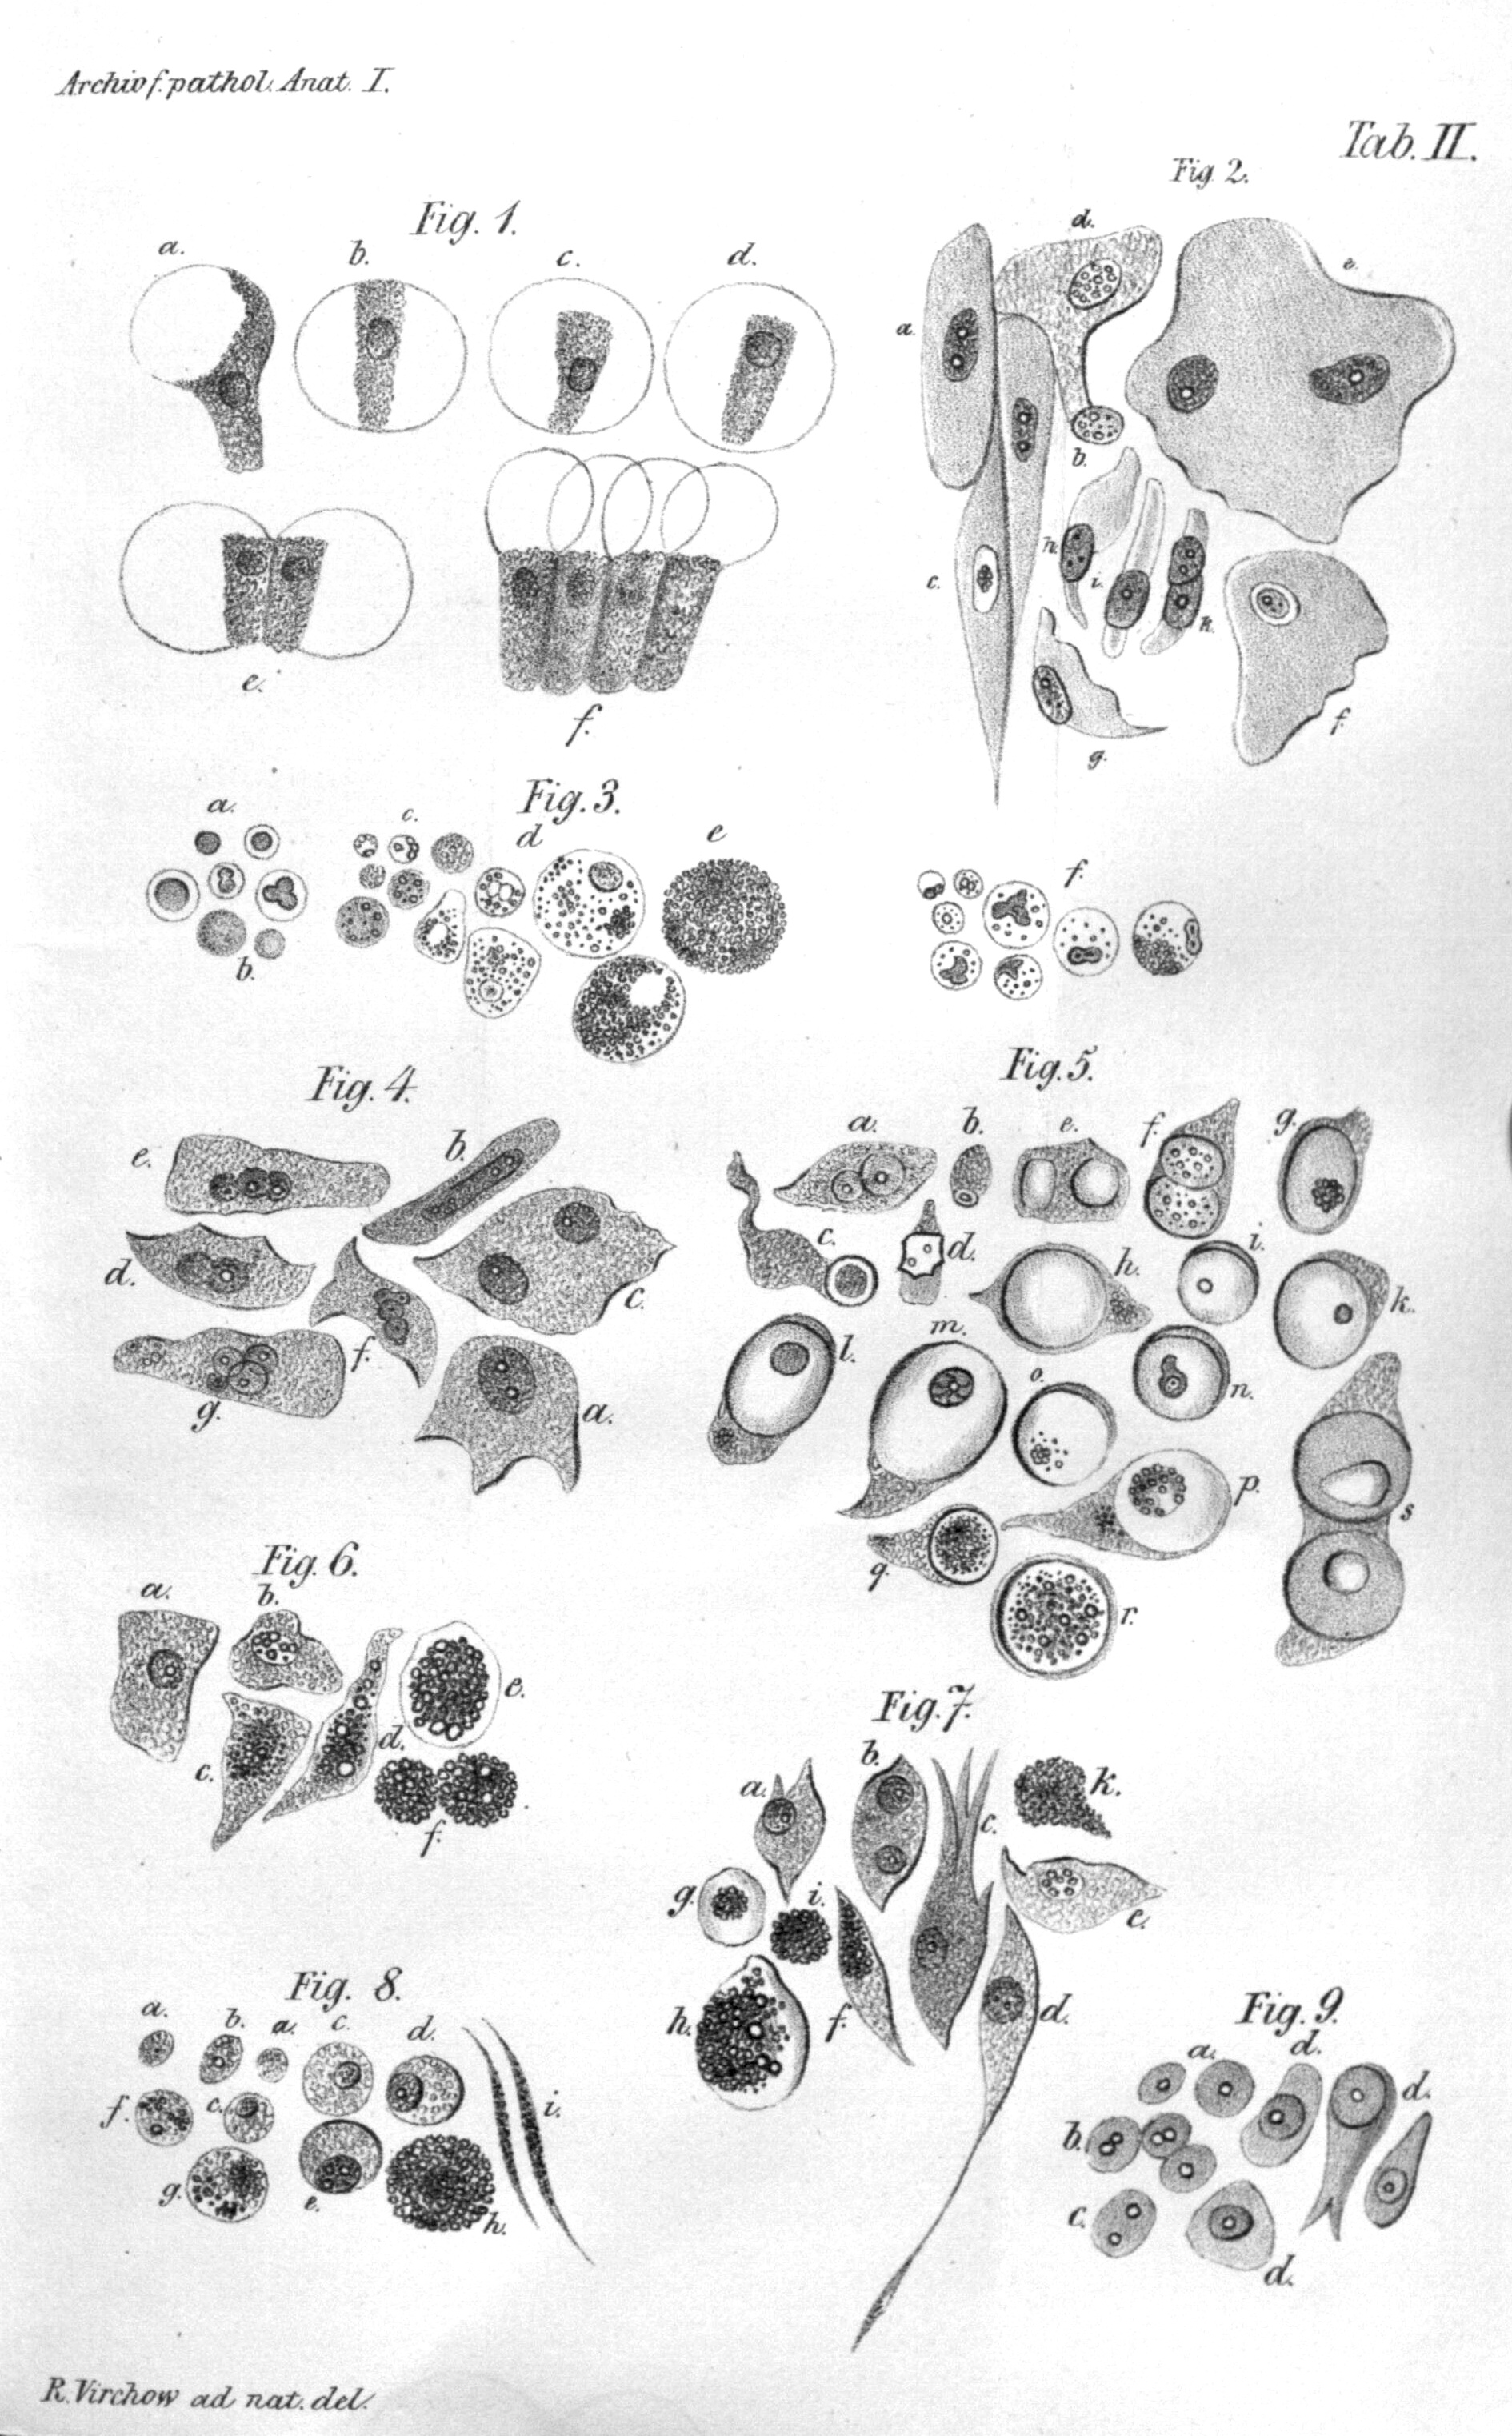
\includegraphics[width=1\linewidth]{figures-ext/01-Virchow-cell} 

}

\caption{\textbf{Illustration of Virchow's cell
theory}. Virchow depicted different cells transformation due to
irritation. \citep{Virchow1847}}\label{fig:Virchow-cell}
\end{figure}





In 1889, Stephen Paget introduced \emph{soil and seed} hypothesis of
metastases \citep{Paget1889}. He formulates it as follows

\begin{quote}
\emph{When a plant goes to seed, its seeds are carried in all
directions, but they can only live and grow if they fall on congenial
soil.}
\end{quote}

Which is a parallel to cancer cells disseminated by body fluids, and
they can grow only tissues - ``soil'' that is predisposed to host the
cancer cell - ``the seed''. He focused on the importance of tissue
characteristics that favorise tumor development as opposed to most
researchers of his time that were focusing on the ``seed'' itself.

In the 20th century, molecular causes started to be investigated. It was
discovered that cancer could be caused by environmental factors,
i.e.~chemicals (carcinogens), radiation, viruses and also inherited from
ancestors. Those factors would damage but contrary to a healthy
condition they would not die.

Also in 1909, Paul Ehrlich, called one of fathers of immunology and
Nobel Prize laureate, indicated a link between immune system and tumor
suppression \citep{Ehrlich1909}. One of remarkable first immontherapy
attempts can be attributed to William Coley, that practiced injecting
streptococcus bacteria directly into patients after cancer surgery in
1891, later called ``Colley vaccine''. However, the impact of this
procedure on patients recovery was judged by scientific community as
``unclear''.

In 1968, Melvin Greenblatt and Philippe Shubik showed that tumour
transplants secete a substance stimulating the growth of blood vessels
\citep{Greenblatt1968}, later identified as ``tumour angiogenic factor
(TAF)'' by Judah Folkman in 1971 \citep{Folkman1971}. Folkman also
suggested that TAF can target of therapy itself which was a revolutional
idea, as it did not target the tumor cells but their environment.

During the 1970s, oncogenes and tumor suppressor genes were discovered.
Oncogenes are genes that allow a cell to become cancer cell, while the
tumor suppressor genes would repair DNA or execute cell death of a
damaged cell. A new dimension to cancer studies was added in the 1980s,
epigenetic changes was proven to occur to both oncogenes and tumour
suppressors \citep{Feinberg1983, Greger1989}, which are presently known
as epigenetic markers used for diagnostics and therapeutic targets for
cancer.

In 1982, Aline van Pel and Thierry Boon \citep{VanPel1982} discovered
that a specific immunity to spontanious tumor cells could be induced by
vaccinating mice with mutagenized tumour cells. This araised an
inspiration for many years of immune therapy developement.

In Napoleone Ferrara and colleagues identified gene encoding vascular
endothelial growth factor (VEGF) that was shown to stimulate growth of
enothelial cells proliferation \emph{in vitro} and angiogenesis (blood
vessels formation) \emph{in vivo} \citep{Leung1989}.

In 1999 for the first time, gene-expression was used to study cancer
(leukeamia) by Todd Golub, Donna Slonim and colleagues
\citep{Golub1999}.

Since the end of the 20th century, cancer screens are developed along
with multiple strategies to fight tumor. Most classical ones are based
on the idea of removing tumor cells (surgery), killing tumor cells with
DNA-blocking drugs (chemotherapy), radiation, inhibit cancer growth
(hormonal therapy, adjuvant therapy and immunotherapy). As non of those
methods is fully efficient, often a combination of treatments is
proposed. Nowadays, science is aming in the direction of trageted
therapies and personalized treatment.

The recent success of immunotherapies (discussed in
\protect\hyperlink{immunotherapies}{Immunotherapies section} attracted
the attention the scientific community again to the context in which
tumor cells are found. This context called Tumor Microenvironment, as
well as the communication that happens within it between different
agents, nowadays studied differently with available knowledge of
molecular biology, have become a popular scientific topics of 21st
century (Fig. \ref{fig:pubmedTME}).

\begin{figure}

{\centering 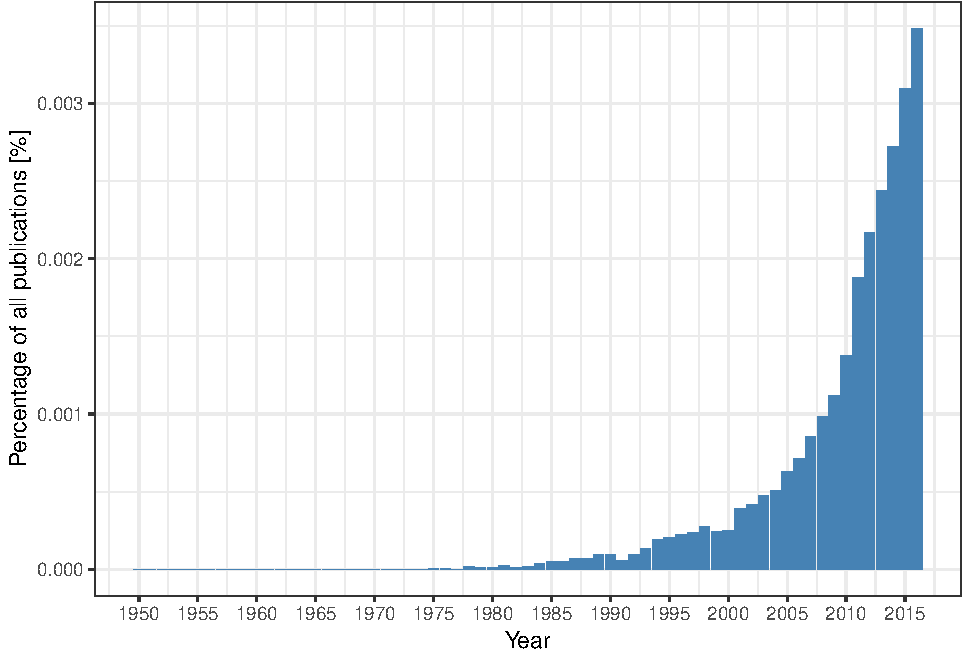
\includegraphics[width=0.7\linewidth]{UCzPhDThesis_files/figure-latex/pubmedTME-1} 

}

\caption{\textbf{Percentage of publications containg
phrase ``tumor immunotherapy'' is growing}, numbers retreived on
17.01.2018 from \href{http://dan.corlan.net/medline-trend.html}{Medline
Trends} \citep{Corlan2004}}\label{fig:pubmedTME}
\end{figure}






\hypertarget{tumor-micro-environment-as-a-complex-system}{%
\subsection{Tumor micro environment as a complex
system}\label{tumor-micro-environment-as-a-complex-system}}

Tumor Microenvironment is a complex tissue that surrounds tumor cells.
It is composed of different compartments (in solid tumors):

\begin{itemize}
\tightlist
\item
  Stroma: blood and lymphatics vessels, epithelial cells, mesenchymal
  stem cells, fibroblast, adipocytes supported by extracellular matrix
  (EM)
\item
  Immune cells: T cells, B cells, NK cells, Dendritic cells,
  Macorphages, Monocytes etc.
\end{itemize}

Their proportion and specific roles vary significantly with tumor type
and stage. Communication between the environmental cells and the tumor
is critical for tumor development and its impact on patient's response
to treatment. These communication between different compartments is
bidirectional and all the players can influence each other. Depending on
the nature and prevailing direction of those interactions different
destiny is possible for each of the compartments, i.e.~immune cells can
be recruited to protect tumor cells or they can kill them directly. Many
of the signals can be contradictory, many can suppress each other. Then
is it possible to tilt this complex ecosystem into patients' favour? Can
we decipher the most important factors of this molecular knot and
manipulate it?

This chapter describes different scenarios of interaction within TME in
order to illustrate the complexity of TME and possible targets for
cancer therapies.

\hypertarget{interactions-between-tme-and-tumor}{%
\subsubsection{Interactions between TME and
Tumor}\label{interactions-between-tme-and-tumor}}

Three scenarios can be considered to describe the relationship between
TME and tumor cells:

\begin{enumerate}
\def\labelenumi{\arabic{enumi}.}
\tightlist
\item
  TME stimulates tumor growth and/or progression and/or impact
  negatively the response to treatment
\item
  TME has no impact on tumor cells and disease development
\item
  TME has a tumor suppressive role and impact positively the response to
  treatment
\end{enumerate}

As can be seen partly in \protect\hyperlink{hist}{Historical
understanding of cancer} these three hypothesis were gaining and loosing
popularity in scientific and medical community over the decades.

\hypertarget{tme-as-a-foe-inflammation}{%
\paragraph{TME as a foe: inflammation}\label{tme-as-a-foe-inflammation}}

In 1863 Rudolf Virchow observed a link between chronic inflammation and
tumorigenesis. According to Virchov theory genetic damage would be the
``match that lights the fire'' of cancer, and the inflammation or
cytokines produced by immune cells should be the ``fuel that feeds the
flames'' \citep{Balkwill2001}. Therefore lymphocyte infiltration was
confirmed by subsequent studies as a hallmark o cancer. The question one
may ask is why our immune system does not defend the organism from tumor
cells as it does in a range of bacterial and viral infections? It is
mainly because of the ability of tumor cells to inhibit immune response
through activation of negative regulatory pathways (so called immune
checkpoints).

Many examples can be cited on how TME facilitates tumor development
(Fig. \ref{fig:met-dis}). For instance, in the early stages of
tumorigenesis some macrophage phenotypes support tumor growth and
mobility through TGF-beta signaling. Also, it was shown that NK cells
and myeloid-derived suppressor cells (MDSCs) have an ability to suppress
immune defence i.e.~immunosurveillance by dendritic cells (DCs), T cell
activation and macrophage polarisation and they promote tumor
vascularisation as well. \citep{Talmadge2013, Gabrilovich2012} They
create so-called niches that facilitates tumor colonization. Tregs and
myeloid-derived suppressor cells can negatively impact natural immune
defence and by these means allow growth and invasion of tumor cells
\citep{Taube2017a}. Another cell type, a part of ECM, fibroblast, or
more precisely Cancer Associated Fibroblasts (CAFs) have proven
pro-tumor functions in breast cancer where they enhance metastasis
\citep{Dumont2013}. The blood and lymphatic vessels maintain tumor
growth providing necessary nutritive compound to malignant cells.

\begin{figure}

{\centering \includegraphics[width=1\linewidth]{figures-ext/massive-dissemination} 

}

\caption{\textbf{The microenvironment supports metastatic
dissemination and colonization at secondary sites.} Different tumor
sites can communicate through exosomes realized by tumor cells and also
immune and stromal cells such as NK cells, CAFs and DCs. Reprinted by
permission from Springer Nature \citep{Quail2013} © 2013 Nature America,
Inc.~All rights reserved.}\label{fig:met-dis}
\end{figure}








According to \citep{Hanahan2012} immune and stroma cells participate in
almost all of Cancer Hallmarks \citep{Hanahan2000, Hanahan2012}. Most of
the hallmarks of cancer are enabled and sustained to varying degrees
through contributions from repertoires of stromal cell types and
distinctive subcell types.

\hypertarget{tme-seen-as-neutral}{%
\paragraph{TME seen as neutral}\label{tme-seen-as-neutral}}

In front of lack of definitive proof that TME can positively or
negatively impact on tumor development, many scientist, in a long time,
ignored the importance of this factor. Until the early-mid eighties, the
TME research was mostly limited to angiogenesis and immune environment
and most areas that are now driving the field were not represented.

From early 70. until the end of the 90. the most accepted statement was
that genetic alterations in oncogenes and tumor suppressor genes are
both necessary and sufficient to initiate tumorigenesis and drive tumor
progression. Therefore TME was not seen as an important element of the
puzzle.

The cancer geneticists, at the time had a lot of influence on scientific
community diminishing the work of made on TME which were considered as
``uninteresting'' and definitely not ``mainstream''.

After 90. with discovery of singling molecules involved in communication
of TME like VEGF. Also discoveries made by developmental biology field
supported the hypothesis that microenvironment plays an important role
in development which was later shown for tumorigenesis. Also success of
immune vaccines starting with the tuberculosis vaccine Bacille
Calmette-Guérin (BCG) in 1976 and finishing, at the moment with
checkpoint inhibitors did not leave the scientific community
indifferent.

\hypertarget{tme-as-a-friend-immunosurveillance}{%
\paragraph{TME as a friend:
immunosurveillance}\label{tme-as-a-friend-immunosurveillance}}

As mentioned in \protect\hyperlink{hist}{Historical understanding of
cancer} Paget proposed a hypothesis of ``seed and soil'' where the TME
in a certain tissue (the soil) can either stimulate or suppress the
metastasis (the seed). William Coley tested a possibility to trigger
tumorsuppressive effect via stimulation of the immune system with
bacteria. In the 1960s, the immune surveillance theory hypothesized
``the ability to identify and destroy nascent tumors as a central asset
of the immune system'' \citep{Sebeok1976, Burnet1970}, but it was highly
criticized in consequence of no increase in tumor incidence in athymic
nude mice \citep{Stutman1974, Rygaard1976}. Later it was shown, that
this mice model was not adequate \citep{Cavallo2011} . Thus, the
hypothesis that TME can have a positive role in tumor prognosis is not
new.

The immunosurveillance through immune-editing can be summarized in three
processes: elimination, equilibrium, and escape \citep{Dunn2002}.

The elimination is direct killing of cancer cells or growth inhibition
by immune system. The adoptive T cells and NK are actively involved in
tumor killing and stimulate other immune cells. The CD8 + cytotoxic
lymphocytes (CTLs) directly recognize tumor cells. Employing perforin-
and granzyme-dependent mechanisms they can lyze tumor cells. The CD4 + T
cells release factors to induce proliferation of B cells and to promote
their differentiation to antibody (Ab)-secreting plasma cells, activate
macrophages. Macrophages use phagocytosis to eliminate cancer cells
\citep{Vesely2011}.

The tumor-infiltrating lymphocytes (TILs) have been associated with an
overall good prognosis and better survival in different cancer studies.
Also, abundance of CD3 + and CD8 + T cells, NK cells, and
\(\gamma\delta\)T cells correlates with improved outcomes in epithelial
ovarian cancers \citep{Marquez-Medina2012}. Several studies report that
the presence of the abundant immune infiltrate is correlated with good
prognosis or better survival
\citep{Kornstein1983, Baxevanis1994, Naito1998, Pages2005}. Spontaneous
regression of human tumors has been reported in cutaneous melanoma,
retinoblastoma, osteosarcoma, etc. \citep{Aris2012}.

The equilibrium is the phase when cancer and immune cells coexist and
their crosstalk is preventing metastasis.

T cells are the main actor maintaining the equilibrium. Progressively,
the tumor cells become more immunogenic as they are not edited by the
immune system \citep{Bahatia2011}. The state of tumor cells is then
identified as ``dormant'' and active scientific reports investigate the
possible molecular pathways that maintain dormancy or lead to escape
\citep{Teng2008}.

The immune escape is the final process when tumor cells impair the
immune response.

\hypertarget{two-faced-nature-of-immune-cells-context-dependent-functional-plasticity}{%
\subsubsection{Two-faced nature of immune cells: context-dependent
functional
plasticity}\label{two-faced-nature-of-immune-cells-context-dependent-functional-plasticity}}

Modern vision of TME-tumor interactions assumes that tumor can be
directed to several molecular pathways. This direction is decided by
signals that are native of tumor cell and/or coming from the
microenvironment.

Recent studies unveil ambivalent nature of immune cells in TME. While
some as cytotoxic T cells, B cells and macrophages can manage to
eliminate tumor cells. Treg cells role is to regulate expansion and
activation of T and B cells. Depending on cancer type, they can be
either pro- or anti-tumor. For example, as it has been shown for T-regs,
usually associated with bad prognosis, they can be associated with
improved survival (i.e.~in colorectal cancer \citep{Frey2010}). For
innate immunity, there are widely accepted M1 (ani-tumor) and M2
(pro-tumor) extreme macrophages phenotypes in TME \citep{Qian2010}. Most
of the statements seem to be context dependent and not valid universally
across all cancer types. We already mentioned Macrophages phenotypic
plasticity as well as different behaviour of EMC depending on tumor
stage.

From more general point of view, it has been observed that
immunodeficiency can correlate with high cancer incidence. Results of
analysis based on observations of 25,914 female immunosuppressed organ
transplant recipients, the tumor incidence was higher than predicted for
multiple cancers. However, the number of breast cancer cases decreased
which can be really disturbing if we need to decide on the role of
immune defence in tumor progression \citep{Stewart1995}. This indicates
that immune microenvironment can be cancer stimulating or inhibiting
depending on the type of cancer and/or other factors.

\hypertarget{immune-cell-subtypes-in-tme}{%
\subsubsection{Immune cell (sub)types in
TME}\label{immune-cell-subtypes-in-tme}}

\begin{quote}
Cette espèce de leucocytes a une grande ressemblance avec certains
éléments fixes du tissu conjonctif, ainsi qu'avec des cellules
endothéliales et des cellules de la pulpe splénique. On est donc souvent
embarrassé, surtout lorsqu'on trouve ces leucocytes mononucléaires en
dehors des vaisseaux, pour les distinguer des autres espèces de cellules
mentionnées.

​ --- Elie Metchnikoff, Leçons sur la pathologie comparée de
l'inflammation, 1891
\end{quote}

Pathological characterisation

FACS molecular charaterisation

Necessary for the chapter \protect\hyperlink{map}{Heterogeneity of
immune cell types}

\hypertarget{summary}{%
\subsubsection{Summary}\label{summary}}

Cancer is a disease concerning milliards of people with a long history.
Scientific community recognises role of the environment where the tumor
cells find themselves as an important factor influencing tumor
development, prognosis and response to treatment. TME is a complex
environment that constantly interacts with tumor cells, where both tumor
and TME influence and shape each other.

Over the years, many interactions are being discovered and cell types
re-defined and described in their context. However, lots of mechanisms
and interactions of TME remains unknown due to very heterogeneous nature
of this micro environment. This leaves room to more extensive
investigation of TME.

A therapeutic goal are target interactions that would be able to pivot
the essential processes in tumorigenesis or tumor escape in order to put
the cells ``back on track'' and facilitate anti-tumor therapies.

These goals can be meet thanks to improvement of investigating
techniques and data quality and abundance. We will discuss the most
important data types used in this project to investigate the TME.

\hypertarget{quantifying-and-qualifying-immune-infiltration-data}{%
\section{Quantifying and qualifying immune infiltration
(data)}\label{quantifying-and-qualifying-immune-infiltration-data}}

Nowadays, more and more biological data is produced. However, this
proliferation of accessible resources is not proportional to generated
insights and wisdom. In this thesis, we wok mostly generate
\emph{Knowledge} and \emph{Insights} and we hope to generate some
\emph{Wisdom} (Fig. \ref{fig:information-power}). In this section, we
will introduce the foundation of our analysis: different data types that
will be further discussed and explored in chapters that follow.

\begin{figure}

{\centering 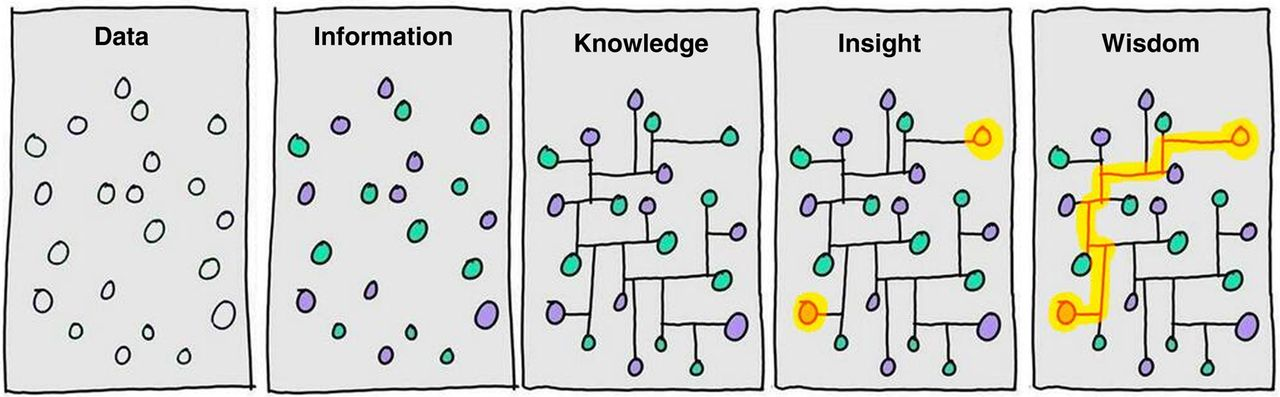
\includegraphics[width=0.8\linewidth]{figures-ext/01-Information_power} 

}

\caption{\textbf{From \emph{Data} to
\emph{Wisdom}}. Illustration of different steps that it takes to go from
\emph{Data} to generating \emph{Wisdom}. It highlights that generating
data is not equal to understanding it and additional efforts are needed
to generate value. Image authored by Clifford Stoll and Gary Schubert
published by Portland Press Limited on behalf of the Biochemical Society
and the Royal Society of Biology and distributed under the
\href{https://creativecommons.org/licenses/by/4.0/}{Creative Commons
Attribution License 4.0 (CC-BY)} in \citep{Ponting2017}.}\label{fig:information-power}
\end{figure}











We will introduce most relevant data types that are used to study immune
infiltration of tumors.

\hypertarget{facs}{%
\subsection{Cell sorting}\label{facs}}

\hypertarget{flow-cytometry}{%
\subsubsection{Flow cytometry}\label{flow-cytometry}}

Flow cytometry is a laser-based technology. It uses marker genes: cell
surface proteins to sort cells in different compartments. Nowadays, it
permits quantification of the abundance of up to 17 cell surface
proteins using fluorescently labelled antibodies \citep{Papalexi2017}.
However this techniques is not free from bias, our knowledge about cell
markers is limited and several markers may not be relevant in some
context. Moreover, the scientific community did not clearly agree on the
marker choice even for popular and well studied cell types which
introduced additional heterogeneity when independent studies are
compared. Also the quality of antibodies may influence the results of
the FACs analysis. Besides those limitations FACs remains quite popular
method for analysing cells in complex tissues. It was among first
methods that allowed molecular phenotyping of immune cells, a discovery
of numerous subsets and thier further functional interpretation.

\hypertarget{mass-cytometry}{%
\subsubsection{Mass cytometry}\label{mass-cytometry}}

Mass cytometry (also known as CyTOF allows for the quantification of
cellular protein levels by using isotopes. It allows to quantify up to
40 proteins per cell \citep{Papalexi2017}. It also demands lower
starting number of cells (1000 - 1000000), a realistic number that can
be extracted from patient biopsy \citep{Lyons2017}.

\hypertarget{staining}{%
\subsection{Microscope Staining}\label{staining}}

Using microscope technics, histopathological cuts are analysed. The
number of cells per a unit of area (i.e.~mm\(^2\)) is defined either
manually by human or though diverse image analysis algorithms. Current
pathology practice utilises chromogenic immunohistochemistry (IHC)
\citep{RamosVara2010}. Multiplexed approaches allow to identify multiple
markers in the same histopathology cut. Modern techniques as imaging
mass cytometry using FFPE tissue samples uses fluorescence and mass
cytometry to identify and quantify marker proteins \citep{Giesen2014}.

The main advantage of aforementioned technics the number of cells that
can be analysed and the information about spatial distribution of the
different cell types. The limiting factor, as for
\protect\hyperlink{facs}{cell sorting methods}, is the number of markers
(\textasciitilde{}10-100) and consequently number of cell types that can
be identified \citep{Schelker2017}.

The \protect\hyperlink{facs}{cell sorting methods} and
\protect\hyperlink{staining}{microscope staining} are usually considered
as a gold standard for multidimensional data techniques. The reason why
they are not applied at large scale is the cost but also quite laborious
and time consuming sample preparation demanding a fresh sample. In
contrast, the \protect\hyperlink{omics}{-omics methods} propose more
scalable way to measure tumor micro environment.

\hypertarget{omics}{%
\subsection{omics}\label{omics}}

\begin{itemize}
\tightlist
\item
  Some kind of sequencing explanation needed for non-biologists
\end{itemize}

\hypertarget{transcriptome}{%
\subsubsection{Transcriptome}\label{transcriptome}}

Transcriptomics measures the number of counts of mRNA molecules using
high-throughput techniques. mRNA is the part of genetic information that
should be translated to proteins. It reflects the activity of ongoing
processes in a cell. In contrast to DNA, mRNA is highly variant
\citep{Velculescu1997}. This variability can be either ``intrinsic''
that reflect the stochastic process or ``extrinsic'' reflecting impact
of factors upstream to mRNA synthesis \citep{Satija2014}.

In addition, many genetic and epigenetic events can be either directly
observed or indirectly inferred from transcriptomic data. Transcriptome
can be measure with microarrays or RNA-seq NGS technology.

Bulk transcriptome data are quite accessible nowadays. They can be
obtained from either flash-frozen or formalin-fixed, paraffin-embedded
(FFPE) tissue samples, including both surgically resected material and
core needle biopsies \citep{Schelker2017}.

The main flaw of transcriptomic data is that the reproducibility between
different platforms is limited. As a result, direct comparison between
two datasets produced by different platforms is not advised.

Different strategies can be adapted to analyse bulk transcriptome.

\citet{Cieslik2017} describes five groups of most popular approaches
that can be applied to study transcriptome (Fig.
\ref{fig:transcriptome-methods}). Despite a diversity of bioinformatic
and statistical tools, the most popular differential approaches, mainly
differential gene expression (DGE) based on difference between two
experimental conditions.

\begin{figure}

{\centering 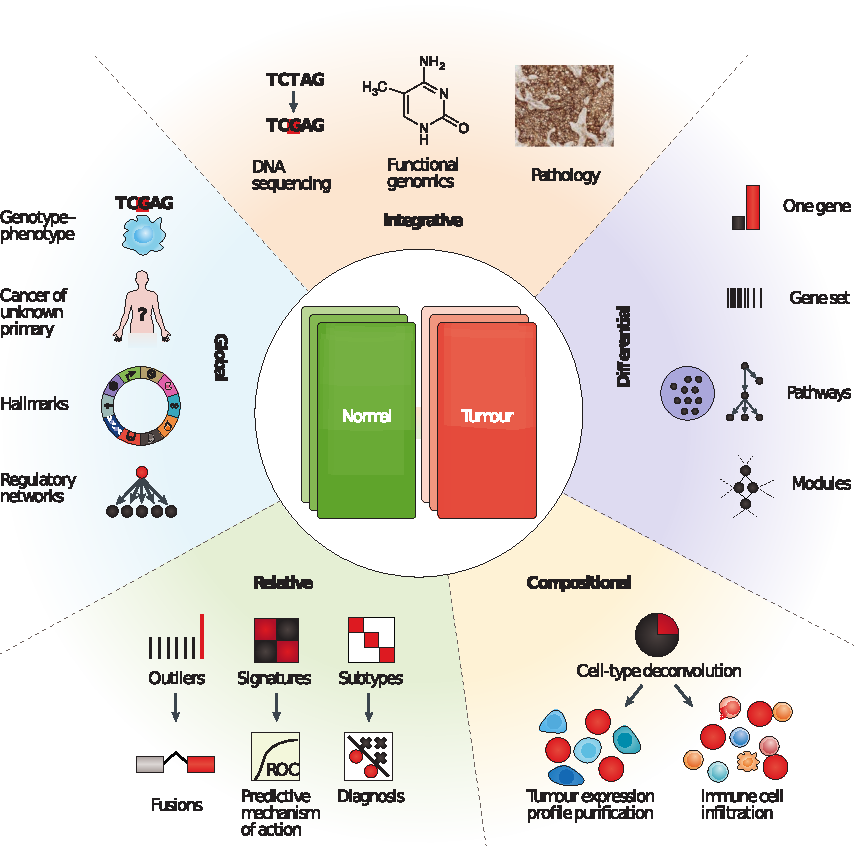
\includegraphics[width=1\linewidth]{figures-ext/transcriptome-methods} 

}

\caption{\textbf{Five categories of RNA-seq
data analysis.} Differential analyses: comparing two (or more)
conditions, Relative analyses: comparing to an internal refernce
(average, base level), Compositional analyses: inferring cell types or
groups of cell types (i.e.~tumor purity), Global analyses: pan-tissue
and pan-cancer analyses and Integrative analyses: compiling
heterogneious data types. Reprinted by permission from Springer Nature
\citep{Cieslik2017} © 2018 Macmillian Publishers Limited, part of
Springler Nature. All rights reserved.}\label{fig:transcriptome-methods}
\end{figure}











RNA-seq data was proven to be a useful indicator for clinical
applications \citep{Mody2015, Oberg2016, Robinson2017}. Its utility for
immune profiling was demonstrated in may studies through a use of
transcriptomic signatures to predict immunotherapy response or survival
\citep{Chen2016}.

In this work transcriptome data analysis fails into multiple categories:
Compositional, Relative and aims to construct a Global-level
conclusions.

\hypertarget{epigenome}{%
\subsubsection{Epigenome}\label{epigenome}}

An epigenome can be defined as a record of the chemical changes to the
DNA and histone proteins of an organism. Changes to the epigenome can
provoke changes to the structure of chromatin and changes to the
function of the genome \citep{Bernstein2007}. Epigenome data usually
contains information about methylation CpG island changes. In cancer,
global genomic hypomethylation, CpG island promoter hypermethylation of
tumor suppressor genes, an altered histone code for critical genes, a
global loss of monoacetylated and trimethylated histone H4 were
observed. Methylome profiles can be also use as molecular signature
\citep{Jeschke2017}.

\hypertarget{single-cell-rna-seq}{%
\subsubsection{Single cell RNA-seq}\label{single-cell-rna-seq}}

Described above methods of process DNA from hundreds of thousands of
cells simultaneously and report averaged gene expression of all cells.
In contrast, scRNA-seq technology allows getting results for each cell
individually. This is tremendous step forward enhancement of our
understanding of cell heterogeneity and opens new avenues of research
questions.

Continuous discovery of new immune subtypes has proven that cell surface
markers that are used for phenotyping by techniques like
\protect\hyperlink{facs}{FACS} and
\protect\hyperlink{staining}{immunohistochelistry} cannot capture the
full complexity. ScRNA-seq methods allow to cluster known cell types in
subpopulations based on their genetic features. ScRNA-seq is also able
to capture particularly rare cell types as it requires much less of RNA
material (1 ng isolated from 100-1000 cells) compared to `bulk' RNA-seq
( \textasciitilde{} 1 μg of total mRNA transcripts ). It also allows to
study cells at high resolution capturing the phenotypes in much more
refined scale than previously \citep{Papalexi2017}.

This new data type also brings into the field new challenges related to
data processing due to the volume, distribution, noise, and biases.
Experts highlight as the most ``batch effect'', ``noise'' and ``dropout
effect'' \citep{Perkel2017}. So far, there are no official standards
that can be applied which makes data comparison and post-processing even
more challenging. Up to date, there are around 70 reported tools and
resources for single cell data processing \citep{Davis2016} .

A limited number of single-cell datasets of tumors are made publicly
available (@ TABLE ?).

One can ask why then developing computational deconvolution of bulk
transcriptome if we can learn relevant information from single-cell
data. Firstly, that single cell data do not provide a straightforward
answer to the estimation of cell proportions. The coverage is not full
and sequenced single cells are not fully representative of the true
population. For instance, neutrophiles are not found in scRNA-seq data
because of they are ``difficult to isolate, highly labile \emph{ex vivo}
and therefore difficult to preserve with current single-cell methods''
\citep{Schelker2017}. In addition, a number of patients included in
published studies of range \textless{}100 cannot be compared to thousand
people cohorts sequenced with bulk transcriptome methods. This is mostly
because single cell experiments are challenging to perform, especially
in clinical setting as fresh samples are needed \citep{Schelker2017}.
Today, single cell technology brings very interesting ``zoom in''
perspective, but it would be incautious to make fundings from a
restricted group of individuals universal to the whole population. Major
brake to the use of single cell technology more broadly might be as well
the price that is nearly 10x higher for single cell sample compared to
bulk \citep{Cedar2018}.

\begin{longtable}[]{@{}cc@{}}
\toprule
Technology & Price\tabularnewline
\midrule
\endhead
scRNA-seq & 3000\$ / sample\tabularnewline
RNA-seq & 200 \$ / sample\tabularnewline
FACS & 0.05\$ / cell\tabularnewline
CyTOF & 35\$/cell\tabularnewline
\bottomrule
\end{longtable}

In this work, we are using single cell data in two ways. Firstly, in
\protect\hyperlink{results}{Chapter 5} we compare immune cell profiles
defined by scRNA-seq, blood and blind deconvolution (problem introduced
in \protect\hyperlink{immune-signatures}{Immune signatures section}).
Secondly, in \protect\hyperlink{map}{Chapter 6} we use single call data
of Metastatic melanoma generated by \citet{Tirosh2016} to demonstrate
heterogeneity of subpopulations of Macrophages and NK cells.

\hypertarget{immunotherapies}{%
\section{From cancer phenotyping to immune
therapies}\label{immunotherapies}}

This section outlines different methods of cancer immune phenotyping and
progress in cancer therapies with a focus on immune therapies. It will
link the ongoing research on TME with therapeutical potential.

\hypertarget{cancer-immune-phenotypes}{%
\subsection{Cancer immune phenotypes}\label{cancer-immune-phenotypes}}

Since 20. century physicians decided on common nomenclature that
classify tumors into distinct groups that are relatively homogenous or
that share common characteristic important for treatment and prognosis.
Tumor typing should help to better asses predicting prognosis, to adapt
a therapy to the clinical situation, to enable therapeutic studies which
are essential in proving any therapeutic progress.

Most of the classifications are based on clinical data. Most common
factors taken into account are: the degree of local invasion, the degree
of remote invasion, histological types of cancer with specific grading
for each type of cancer, possibly various tumour markers, general status
of the patient.

However, cancers with similar morphological and histopathological
features reveal very distinct patterns of progression and response to
therapy \citep{Galon2014}. In the era of gene sequencing, gene and
protein expression as well as epigenome can provide an important
complementary information. Therefore gene markers or proteomic
abnormalities can integrated into classification panel. One popular
example is a gene signature \emph{PAM50} \citep{Parker2009} used for
prediction of patients' prognosis in breast cancer, patented as a tumor
profiling test.

Since the increase of importance of the immunotherapies, researches
proposed several ways to classify tumors based on their
microenvironment. Given different parameters describing TME, cancers can
be sorted into groups that show similar characteristics. We will discuss
most common frameworks that allow to phenotype cancers based on the TME.

The localisation of the immune cells can be an indicator of the state
and response to the therapy \citep{Bindea2013}.

The most standard approach is to convey an analysis of histopathological
cuts to asses the number of infiltrating lymphocytes (TILs). Two typical
patterns are usually identified: ``hot'' - immune inflamed and ``cold''
- no active immune response \citep{Berghoff2018}.

\citet{Chen2017} describes classification into inflamed and non-inflamed
tumors, where non-inlamed phenotypes: can be further split into the
immune-desert phenotype and the immune--excluded phenotype (Fig.
\ref{fig:immune-phenotypes}). The inflamed phenotype is characterised by
rich presence of immune cells : T cells, myeloid cells, monocytes in
tumor margin. Along with the immune cels, due to their communication, a
high expression of cytokines is characteristic for this phenotype.
According to Chen2017, this is a mark of anti-tumor response that was
arrested by tumor. The inflamed phenotype has shown to be most
responsive to immunotherapies. In the immune-excluded phenotype, the
immune cells are present as well but located in the stroma
\citep{Herbst2014}, sometimes penetrating inside tumor. However, when
exposed to check point immuotherapy, T cells does not gain the ability
to infiltrate the tumor, therefore the treatment is inefficient. The
immune-desert main features is little or no presence of immune cells,
especially T cells. Surprisingly, this tumors have been to proven to
rarely respond to the checkpoint therapy \citep{Herbst2014}. In
non-inflamed tumours cytokines associated with immune suppression or
tolerance are expressed.

\begin{figure}

{\centering 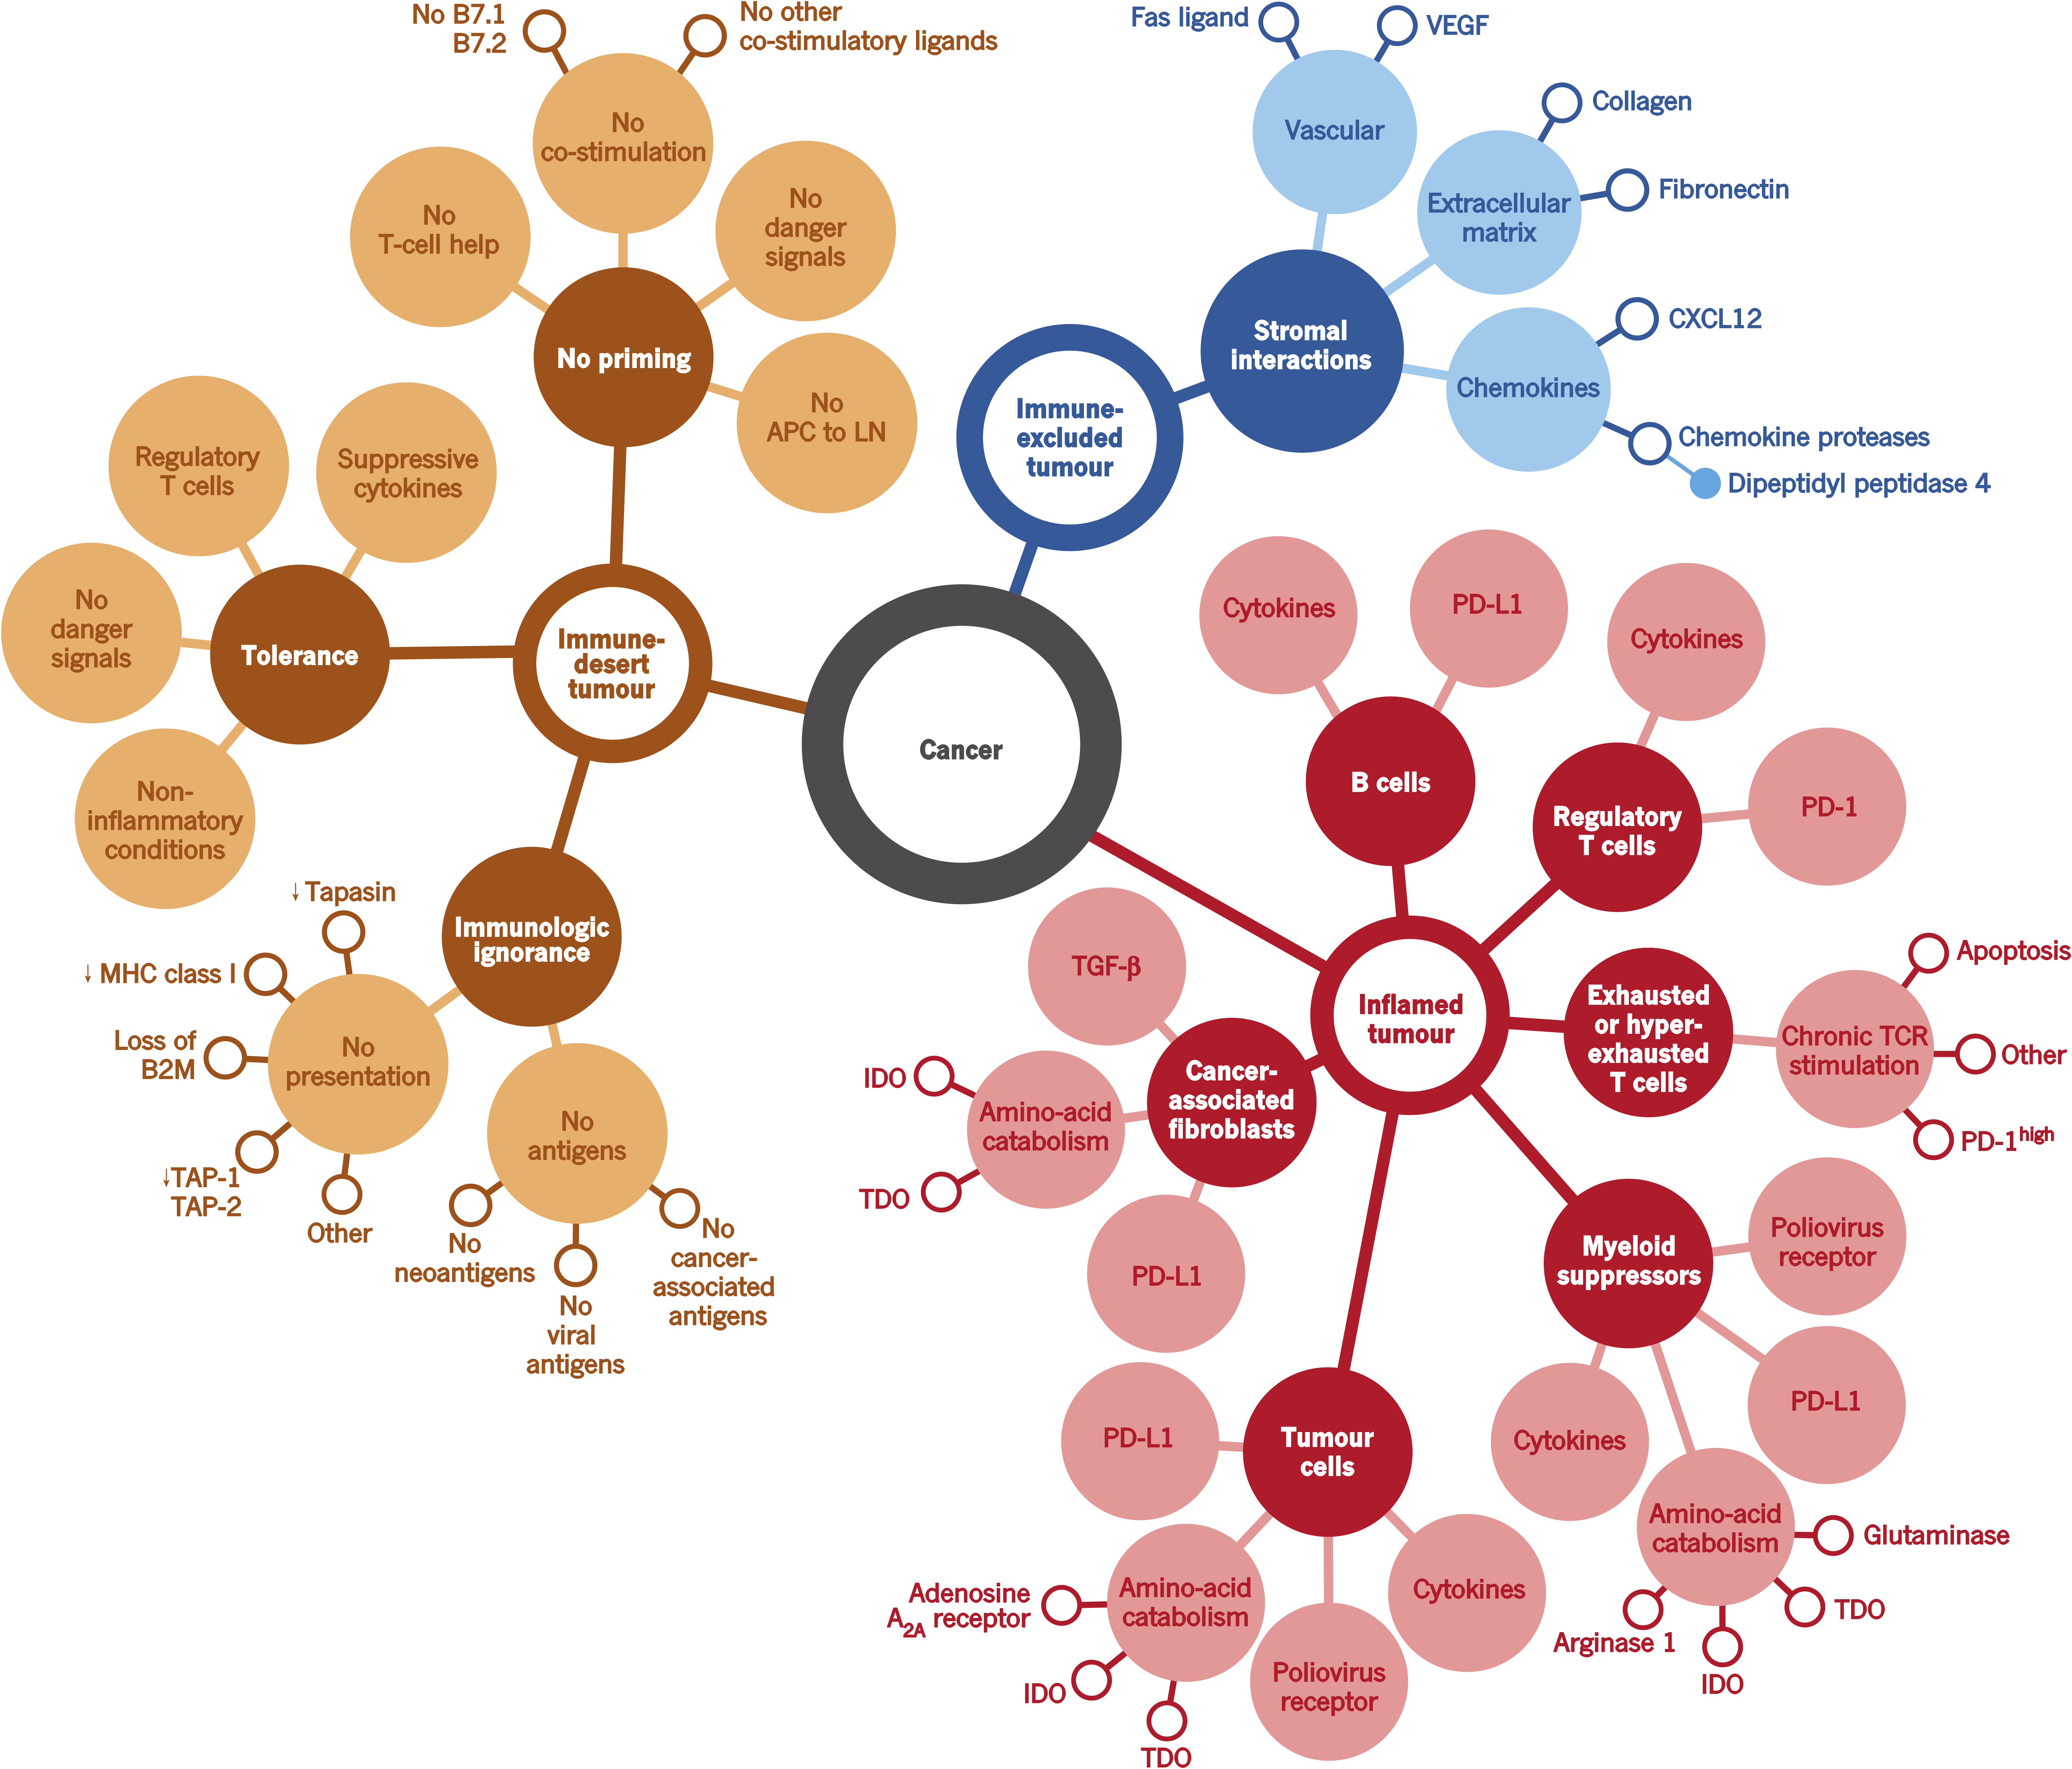
\includegraphics[width=1\linewidth]{figures-ext/immune-phenotypes} 

}

\caption{\textbf{Cancer-immune phenotypes: the
immune-desert phenotype (brown), the immune--excluded phenotype (blue)
and the inflamed phenotype (red).} The immune--desert phenotype is
characterised by paucity of immune cells and cytokines. In the
immune-excluded phenotypes the T cells are often present but trapped in
stroma, enabled to migrate to the tumor site. The immune-inflamed
phenotype is rich in immune cells and the most responsive to the immune
check point therapies. Reprinted by permission from Springer Nature
\citep{Chen2017} © 2017 Macmillian Publishers Limited, part of Springler
Nature. All rights reserved.}\label{fig:immune-phenotypes}
\end{figure}












\citet{Thorsson2018} performed a multi-omic analysis of TCGA datasets
that allowed them to define 6 subtypes that are valid across cancer
types:

\begin{enumerate}
\def\labelenumi{\arabic{enumi}.}
\tightlist
\item
  wound healing
\item
  IFN-\(\gamma\) dominant
\item
  inflammatory
\item
  lymphocyte depleted
\item
  immunologically quiet
\item
  TGF-\(\beta\) dominant
\end{enumerate}

Different indicators were used to define these six phenotypes:

The immunogenicity of the tumors can be explained by tumor-intrinsic
factors and tumor-extrinsic factors \citep{Gajewski2006}.
Tumor-intrinsic factors are, the neoantigen load and frequency, the
mutational load, the expression of immunoinhibitors and
immunostimulators (e.i. PD-L1), and alteration of HLA class I molecules.
Tumor-extrinsic factors include chemokines regulating T cell
trafficking, infiltration of effector TILs and immunosuppressive TILs,
and soluble immunomodulatory factors (cytokines).

A plethora of different computational methods have been developed in
order to further characterize tumor samples using different factors. We
mention here mainstream methods that cover different approaches of
scoring the TME-cancer phenotype.

\hypertarget{immunoscore}{%
\subsubsection{Immunoscore}\label{immunoscore}}

One of the most recognised scoring method, based on fluorescent images
is authored by Jerôme Galon lab in Paris and names
\href{http://www.haliodx.com/clinical-research-services/immunoscorer/}{Immunoscore}.
The Immunoscore ranges from 0 to 4 and it is based on the density of
lymphocyte populations CD3/CD45RO, CD3/CD8, or CD8/ CD45RO. It also
takes into account the spacial position of the cells: the tumor core and
margins \citep{Galon2012}. It was successfully applied to colorectal
cancer to predict patients' survival \citep{Anitei2014} . Since it
resulted in numerous application to many cancer types. It was also
linked to time-to-recurrence in an international study. There is great
potential to use immunoscore as a predictive marker if validated in
prospective studies \citep{Galon2016}.

The immunoscore is an interesting indicator, especially in the scope of
clinical applications, although it does not tell us a lot about
underlying biology. It is also limited to a few cell types while it may
be that in some cancer types or patients, the system requires more
detailed or rich analysis of larger panel of cells.

\hypertarget{immunophenoscore}{%
\subsubsection{Immunophenoscore}\label{immunophenoscore}}

Different approaches are based on gene expression patterns. Most
commonly, machine learning supervised algorithms are trained to match
known phenotype (established with microscopy or with clinical features)
to genetic patterns or an unsupervised clustering is used to discover
new classification.

An example of well-formulated classification framework is
Immunophenoscore \citep{Charoentong2017}, based on publication of
\citet{Angelova2015}, where methylome, transcriptome and mutation of
TCGA CRC dataset (n = 598) was used to describe \emph{immunophenotypes}.
Later on, it was reduced to gene expression indicator and summarised in
a form of a score. In This scoring scheme is based on the data of 20
solid tumors, using expression of marker genes selected by a Machine
Learning algorithm (random forest) for best prediction in each cancer.
These indicators can be grouped into four categories:

\begin{itemize}
\tightlist
\item
  MHC molecules (MHC)
\item
  Immunomodulators (CP)
\item
  Effector cells (EC)
\item
  Suppressor cells (SC)
\end{itemize}

The immunophenscore (IPS) is calculated on a 0-10 scale based on the
expression of genes in each category. Stimulatory factors (cell types)
impact the score positively and inhibitory factors (cell types)
negatively. Z-scores ≥ 3 were designated as IPS10 and z-scores ≤ 0 are
designated as IPS0. A similar conceptual framework called \emph{cancer
immunogram} was proposed by \citet{Blank2016} included seven parameters:
tumor foreignness (Mutational load), general immune status (Lymphocyte
count), immune cell infiltration (Intratumoral T cells), absence of
checkpoints (PD-L1), absence of soluble inhibitors (IL--6, CRP), absence
of inhibitory tumor metabolism (LDH, glucose utilisation), tumor
sensitivity to immune effectors (MHC expression, IFN-γ sensitivity).
\citet{Charoentong2017} claim that the immunophenoscore can predict
response to CTLA-4 and anti-PD-1.

Nonetheless, the details of \emph{cancer immunogram} use in practice
remain unclear and result could be sensitive to patients' and data
heterogeneity as no standardisation was proposed. It should be also
validated in a systematic independent study.

\hypertarget{immune-maps}{%
\subsubsection{Immune maps}\label{immune-maps}}

Another way to summarize tumor phenotype can be though use of molecular
maps. \href{https://acsn.curie.fr/}{Atlas of Cancer Signaling Network
(ACSN)} \citep{Kuperstein2013, Kuperstein2015} is primarily a~pathway
database that contains a collection of interconnected cancer-related
signalling network maps. An additional feature is ACSN web-based
goole-maps like visualisation of the database. User data can be
projected on the molecular map (for example gene/protein expression from
user data can be paired with entities on the map ). Currently it
contains \href{https://navicell.curie.fr/}{11 maps} covering signalling
processes involved in apoptosis, cell cycle, DNA repair, EMT, cell
motility, Ewing sarcoma, Dendritic cells, Macrophage cells, Natural
killer cells, CAF and integrated innate immunity map. Through projection
of the data on the innate immunity map, one can see if the patient or a
sample is characterised by pro- or anti-tumor activated pathways due to
the organisation of the map layout. Also, different CAF subtypes were
characterised with the CAF specific map in \citep{Costa2018}. Kondratova
and colleagues (including myself) used innate immune map to characterize
NK and Macrophages subtypes and in another publication
\citep{Kondratova2018} different patient profiles using scRNAseq data of
Metastatic melanoma.

\hypertarget{summary-1}{%
\subsubsection{Summary}\label{summary-1}}

Despite those facts, the gene expression based classifications are not
yet used in clinics. The measured multi-panel mRNA expression, that can
be included into category of In Vitro Diagnostic Multivariate Index
Assay (IVDMIA) \citep{Gyorffy2015, Ross2008}, may be a future of
TME-based cancer classification, diagnosis and treatment recommendation
\citep{Gnjatic2017}. For this best tools need to be used to properly
evaluate the state of TME and tumor-stroma-immune cells communication.

\hypertarget{immune-signatures}{%
\subsection{Immune signatures - biological
perspective}\label{immune-signatures}}

\begin{itemize}
\tightlist
\item
  definition of signature: marker genes, list of genes, weighted list,
  metagenes
\item
  the general immune signature of signature of immune infiltration and
  stroma vs immune signature of a specific cell type of functional
  subpopulation
\item
  purpose of signatures
\item
  availability of immune signatures
\item
  the problem of not consistency of immune signatures
\item
  origin of signatures
\end{itemize}

\begin{quote}
\emph{the gene expression profiles of tumour-associated immune cells
differ considerably from those of blood derived immune cells}
\citep{Schelker2017}
\end{quote}

Immune signatures will be also discussed as a part of deconvolution
pipeline in the \protect\hyperlink{methods}{Chapter 2} under the section
about \emph{basis matrix}.

---------

Gene expression signatures

Lack of immune-specific signatures. Gene expression signatures are used
as tools to predict which patients will benefit from certain treatments
and to guide decision-making in the clinic.46

Gene expression signatures are considered ``prognostic'' when they can
differentiate between patients with a good or bad prognosis in the
context of traditional therapy or no treatment at all.47 Gene signatures
are considered ``predictive'' when they are able to predict treatment
benefit between experimental and/or nontraditional treatment groups
vs.~control, typically in the setting of a randomized controlled
clinical trial.47 In breast cancer, the predictive and prognostic assays
Oncotype DX, EndoPredict, PAM50, and Breast Cancer Index are now
recommended as adjuncts for clinical decision-making for patients with
specific subtypes of breast cancer.46 These signatures, however, are not
specifically immune-related and share little overlap in their selected
genes.47, 48 Because tumor cells and infiltrating immune cells both have
prognostic value, evaluating tumors and the surrounding stroma with use
of the methods described above, in order to generate immune-related
signatures, can provide prognostic and perhaps predictive information
associated with patient outcome. Although there are no immune-related
gene signatures used in clinical practice currently, several studies
have shown the validity and reproducibility of using immune-related
signatures to predict outcome and response to therapy in patient cancer
samples.

Solution: in silico, pan-cancer studies. One reason immune-related gene
signatures have not been widely used in clinical settings is the lack of
consistency of genes, both within the same tumor type and among
different tumors.49 Efforts to address this problem are under way, with
the development of conserved immune gene signatures representing
multiple tumor types.49 Another problem with immune-related gene
signatures is the difficulty in decipher- ing whether the genes
represent specific immune cell popula- tions, antigen-presenting
machinery, cytokines, or other immune- related molecules. In silico
studies have validated pan-cancer immune-related gene signatures that
represent many immune cell types with known prognostic significance
including T cells, B cells, NK cells, macrophages, as well as various
cytokine populations.49, 50 Immune-related gene signatures have proven
to be prognostic of clinical outcome across multiple cancer types and
are associated with response to immune therapy in specific cancers.49,
50 Recent findings on immune-related gene signatures have shown that
gene signatures are able to distinguish between broad lineages of cell
type, such as lymphoid and myeloid but are less adept at distinguishing
between more differentiated cells such as CD8+ and CD4+ T cells.49

Ranked gene lists

Oversimplification of interpretation. Currently, given the multi-

tude of methods with which to analyze genomic data, the

problem no longer lies in obtaining gene expression profiles but

rather in interpreting the data. Analysis of gene expression data

typically involves a comparison of two groups and the creation of

a ranked gene list based on expression. One method of

interpretation involves looking at each end of the ranked list to

7, 51

Quantity of data. The NCBI Gene Expression Omnibus database contains
more than 30,000 series and 1 million samples of array- based expression
data, many of which involve the immune system.52 Because of the large
amount of expression data relating to the immune system and the
inability to compare information between the various datasets, the
Immunological Genome Project (IGP) was created to provide a
comprehensive compendium of the expression of protein-coding genes for
all immune cell popula- tions in the mouse immune system.53 This project
was developed to provide information on primary immune cells isolated ex
vivo from the mouse immune system and then integrate that information
into networks, while taking into account variation via genetic
polymorphisms, knock-out of genes, knockdown via RNA interference, and
drug treatment.53 Researchers can use these data to determine gene
expression profiles that serve as biomarkers for predicting response to
treatment and for measur- ing residual disease after immune therapy.

Solution 1: added-value/specialty databases. Primary databases contain
gene expression and other genomic data such as genotype, DNA
methylation, and protein expression data. These

evaluate genes showing the largest difference in expression. Problems
with this method include small relevant biological differences between
genes leading to no statistical significance, a long list of genes that
are statistically significant but lack biologic relevance, missed
effects on pathways by analyzing single genes, and variation in gene
lists for the same biologic system based on two different groups'
data.51 This again underscores the challenge faced when trying to create
a clinically useful immune-related gene signature from a high-throughput
panel of genes.

\citet{Lyons2017}

-------

\hypertarget{cancer_Therapies}{%
\subsection{Cancer therapies}\label{cancer_Therapies}}

Cancer is a complex disease. Up to date, no uniform and fully effective
treatment was proposed and usually different strategies are tested to
kill tumor cells. \textbf{Surgery} is one of the oldest methods. The
cancer is removed from the patient body. There are different ways, more
or less invasive, that it can be performed. it is usually applied for
solid tumor contained in a small area. \textbf{Radiation Therapy} uses
high doses of radiation to eliminate tumor cells and shrink tumor mass.
It can be applied externally or internally. \textbf{Chemotherapy} uses a
drug (or a combination of drugs) that kill cancer cells, usually
altering cell proliferation and growth. The drawback of radiotherapy and
chemotherapy are strong side effects. \textbf{Hormone therapy } modulate
hormone levels in the body in order to inhibit tumor growth in breast
and prostate cancers. In leukemia and lymphoma, can be applied
\textbf{stem cell transplants} that restore blood-forming stem cells
destroyed by the very high doses of chemotherapy or radiation therapy
that are used to treat certain cancers.

Alternatively, \textbf{targeted therapies} represent more focused
strategy that aims to be more effective and cause less side effects than
systematic therapies. Two main types of targeted therapies are
small-molecule drugs and monoclonal antibodies. Targeted therapies
usually aim to stimulate/inhibit a selected molecular function. A
special types of targeted therapies are \textbf{Immunotherapies}.
Through adtivation/inhibition of immune regulatory pathways, it
stimulates immune system to destroy malignant cells. A continuation of
targeted therapies is \textbf{precision medecine approach}. It is based
on genetic information to specify patient's profile and find adapted
treatment. A number of innovative treatments targeting a specific change
in tumor ecosystem are being tested presently in precision medicine
clinical trials \citep{NCI2018}.

\hypertarget{recent-progress-in-immuno-therapies}{%
\subsection{Recent progress in
immuno-therapies}\label{recent-progress-in-immuno-therapies}}

The immunotherapies, in contrast with other types of cancers therapies
discussed in \protect\hyperlink{cancer_Therapies}{the previous chapter},
aim to trigger or restart the immune system to defend the organism and
attack the malignant cells. All this, however without provoking
persisting inflammation state \citep{Predina2013}

The idea of stimulating immune system to fight malignant cell was not
born recently. Since a long time a possibility of development of an
anti-cancer vaccine has been investigated. Unfortunately, this idea
faced two important limitations 1) lack of knowledge of antigens that
should be used in vaccine to successfully stimulate cytotoxic T cells 2)
the ability of cancer to block the immune response also called
\emph{immunostat}. Despite those impediments works on anti-tumor
vaccines do not cease \citep{Palucka2013}. A very recent promising an
in-situ ani-tumor vaccine was proposed by Sagiv-Barfi et al.
\citep{Sagiv-Barfi2018}. The therapy tested in mice, would be based on
local injections of the combination of ``unmethylated CG-enriched
oligodeoxynucleotide (Cp-G) - a Toll-like receptor 9 (TLR9) ligand and
anti-OX40 antibody. Low doses of CpG injected into a tumor induce the
expression of OX40 on CD4+ T cells in the microenvironment in mouse or
human tumors. An agonistic anti-OX40 antibody can then trigger a T cell
immune response, which is specific to the antigens of the injected
tumor''. Sagiv-Barfi et al.~claim this therapy could be applied to all
tumor types, as long as they are leucocyte-infiltrated. As a local
therapy, in situ vaccination should have less side-effects than
systematic administration. It is now undergoing clinical trials to test
its efficiency in human patients.

Another idea involving using immune system as a weapon to fight cancer,
would be the use of genetically modified patient's T-cells, carrying
\emph{CARs} (chimeric antigen receptors) \citep{Jackson2016}. After a
long period of small unsuccessful trials, recently in 2017, two CAR
T-cell therapies were accepted, one to ``treat adults with certain type
of large B-cell lymphoma'' \citep{FDACARTadult}, other to treat
``children with acute lymphoblastic leukemia (ALL)'' \citep{FDACARTALL}
, which are, at the same time, the first two gene therapies accepted by
FDA.

However, the two most promising immuno-related strategies with proven
clinical efficiency are based on blocking so called immune check point
inhibitors: cytotoxic T-lymphocyte protein 4 (CTLA4) and programmed cell
death protein 1 (PD-1). The anti-CLTA4 antibodies blocks repressive
action of CLTA4 on T-cells and they become therefore activated. It was
shown efficient in melanoma patients and accepted by FDA in 2015 as
adjuvant therapy for stage III metastatic melanoma patients
\citep{FDACTLA4}. PD-1 is a cell surface receptor of T cells, that binds
to PD-L1/PD-L2. After binding, an immunosuppressive pathway is activated
and T cells activity is dampened. An action of an anti-PD-L1 antibody is
to prevent this immune exhaustion \citep{Chen2017}. A stepping stone for
anti-PD-L1 therapies was approval of Tecentriq (atezolizumab) for
Bladder cancer \citep{FDAPDL1Bladder} and anit-PD1 Keytruda
(pembrolizumab) initially accepted for NSCLC and further extended to
head and neck cancer, Hodgkin's lymphoma, gastric cancer and
microsatellite instability-high cancer \citep{FDAPDL1NSCLC}. Since other
anti-PD-L1 or anti-PD1 antibodies were accepted or entered advanced
stages of clinical trials \citep{Wolchok2015}. A short history of
immunotherapy FDA-accepted treatments can be found in Fig.
\ref{fig:timeline-immunotherapies}

\begin{figure}

{\centering 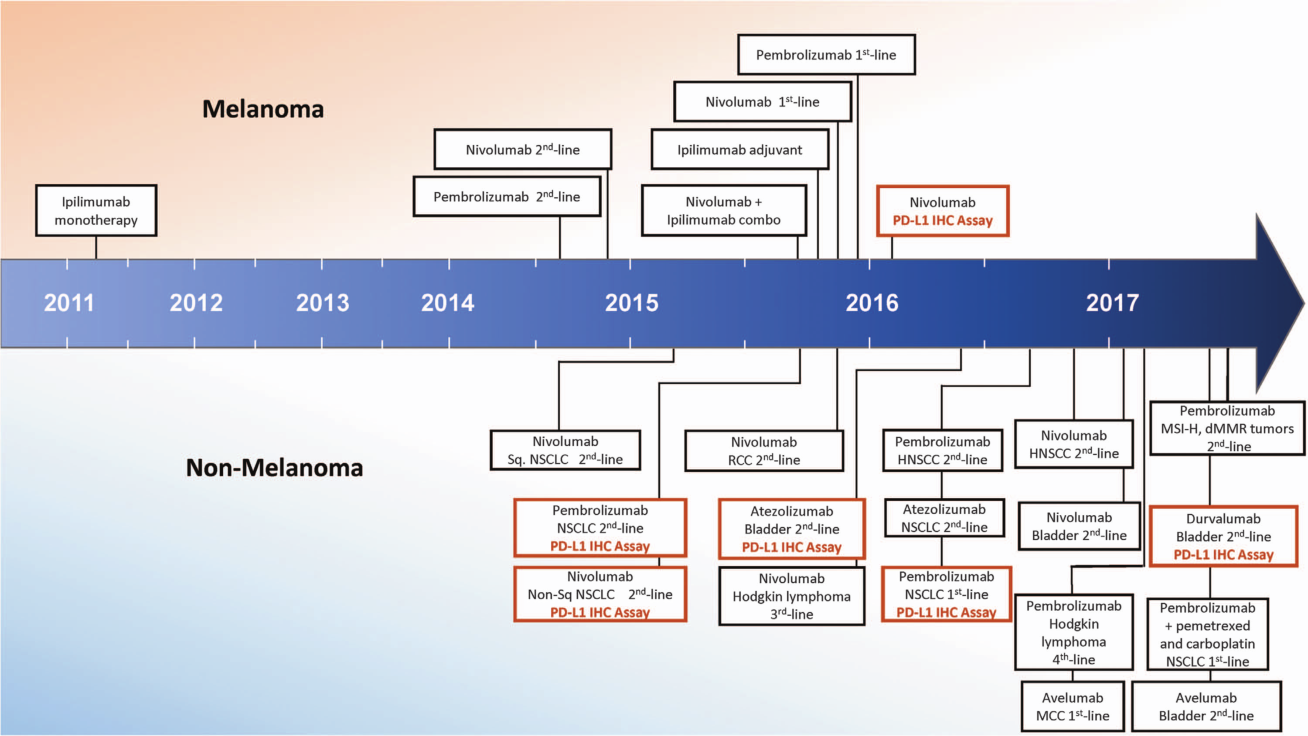
\includegraphics[width=1\linewidth]{figures-ext/02-timeline-immunotherapies} 

}

\caption{\textbf{This timeline describes
short history of FDA approval of checkpoint blocking immunotherapies up
to 2017.} Reprinted by permission from Springer Nature
\citep{Taube2017a} Macmillan Publishers Limited, part of Springer
Nature. All Rights Reserved.}\label{fig:timeline-immunotherapies}
\end{figure}







The main drawback of immunotherapies is a heterogeneity of response
rate, which can vary i.e.~from 10--40\% in case of PD-L1blocking
\citep{Zou2016}, suggesting that some patient can have more chances than
others to respond to an immune therapy. So far, it has been shown that
anti PD-L1 therapies works more effectively in T cell infiltrated tumors
with exclusion of Tregs because of lack of difference in expression of
FOXP3 in responding and non-responding group of patients
\citep{Herbst2014}. Also some light has been shade by \citet{Rizvi2015}
who connected mutational rate of cancer cells to the chances of response
to an immunotherapy.

Despite those fundings, the precise qualifications of patients that
should be sensitive to an immunotherapy are not defined
\citep{Pitt2016}. As most patients do not answer to immunotherapies, it
stimulates researches to look for better biomarkers and patient
stratifications, and pharmaceutical industries to discover new immune
checkpoints based therapies.

\hypertarget{biological-dimension-of-the-thesis}{%
\section{Biological dimension of the
thesis}\label{biological-dimension-of-the-thesis}}

Explaining the biological dimension of the project

\begin{itemize}
\tightlist
\item
  help to better understand tumor immunophenotypes (cell types present
  and their biology, interactions)
\item
  propose predictive biomarkers - precision medecine
\item
  better explore available data
\item
  integrate the data (transcriptome \& methylome, validate transcriptome
  with FACS etc.)
\end{itemize}

\hypertarget{methods}{%
\chapter{Mathematical foundation of cell-type deconvolution of
biological data}\label{methods}}

In this chapter, we will discuss how mathematical models can be used to
extract information about specific cell-types from `bulk' data or how to
unmix mixed sources. It will introduce you to basic concepts of data
analysis as well as most popular advanced solutions adapted for
estimating presence and proportion of immune cells within cancer
biopsies.

\emph{Note: Parts of this chapter with benchmark data might be a part of
a future review}

Explain the principle

\begin{figure}

{\centering 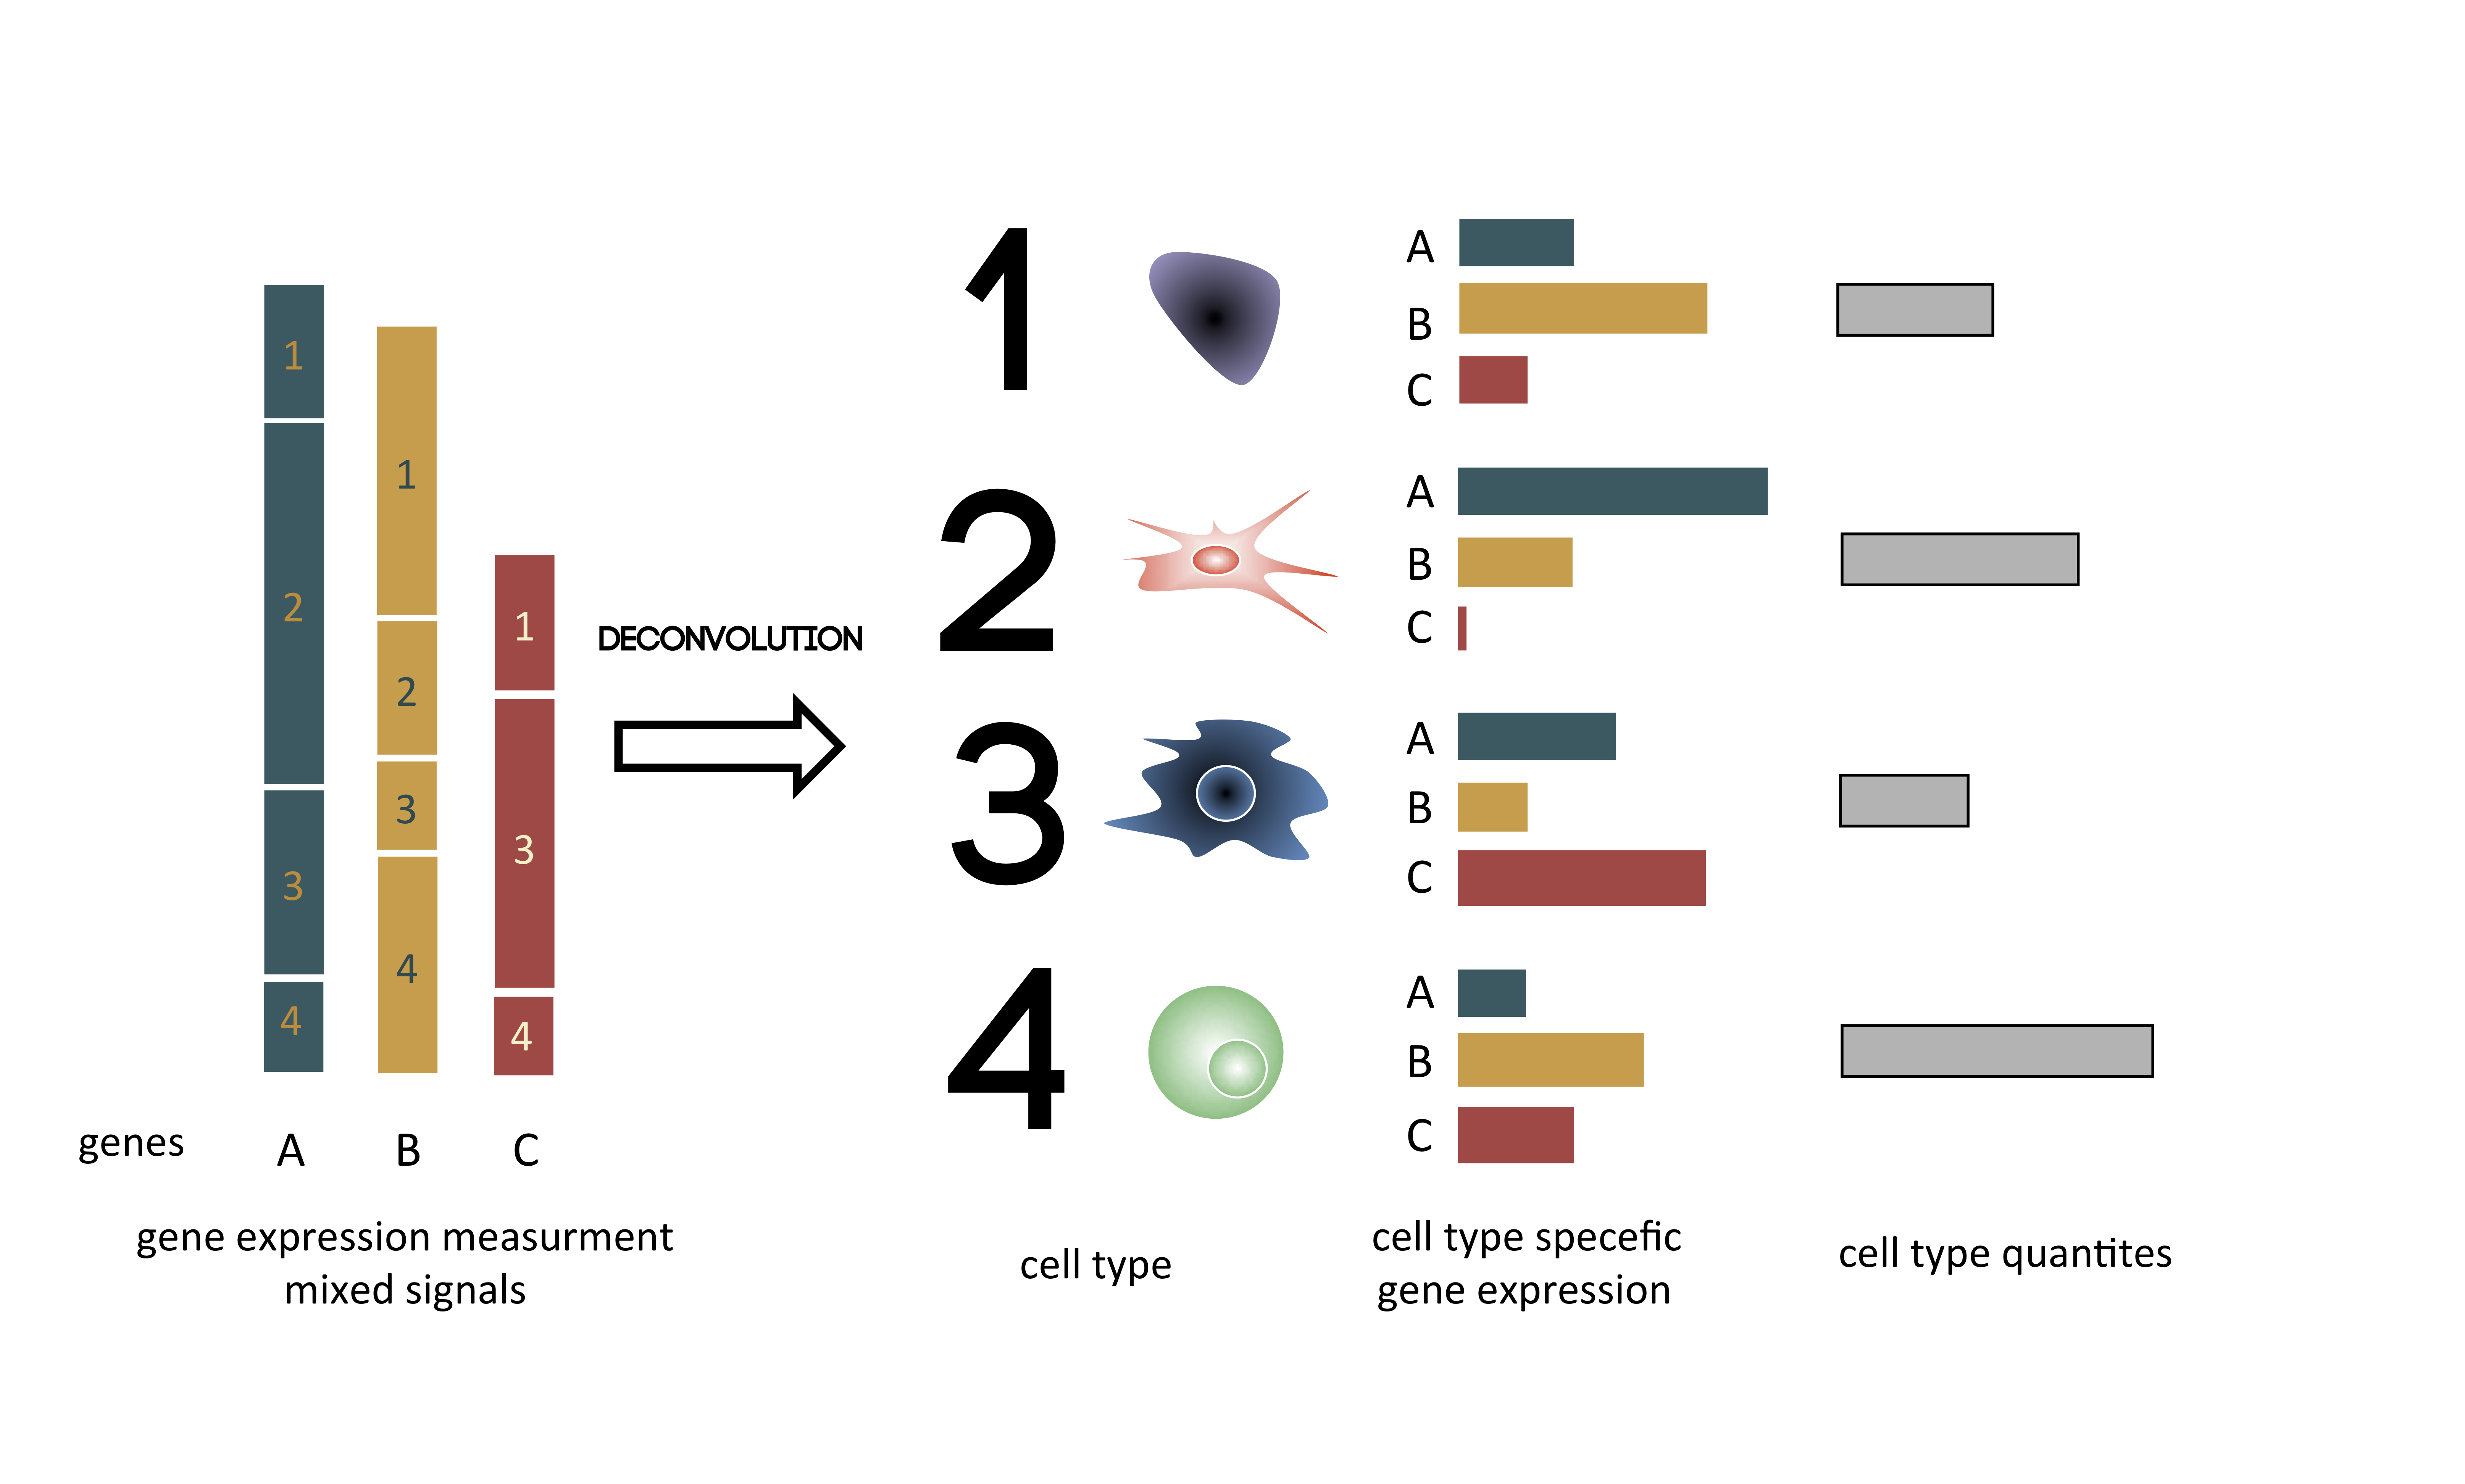
\includegraphics[width=1\linewidth]{figures-ext/deconv} 

}

\caption{\textbf{Principle of the
deconvolution applied to transcriptome} Graphical illustration of the
deconvolution of mixed samples. Starting from the left, gene expression
of genes A B C is a sum of expression of cell types 1, 2, 3, 4. After
deconvolution, cell types are separated and gene expression of each cell
type is estimated taking into account cell type proportions.}\label{fig:deconvolution-cartoon}
\end{figure}








\hypertarget{introduction-to-supervised-and-unsupervised-learning}{%
\section{Introduction to supervised and unsupervised
learning}\label{introduction-to-supervised-and-unsupervised-learning}}

\begin{itemize}
\tightlist
\item
  Explaining difference between supervised and non-supervised learning
  technically and in our context
\end{itemize}

\hypertarget{blind-source-separation}{%
\section{Blind source separation}\label{blind-source-separation}}

(ICA, NMF, CAM)

\hypertarget{finding-optimal-number-of-components-and-over-decomposition-of-transcriptopmes}{%
\section{Finding optimal number of components and over-decomposition of
transcriptopmes}\label{finding-optimal-number-of-components-and-over-decomposition-of-transcriptopmes}}

\begin{itemize}
\tightlist
\item
  Explain why this problem is important
\item
  Explain shortly my role in the paper
\end{itemize}

\citep{Ulykbek2017}

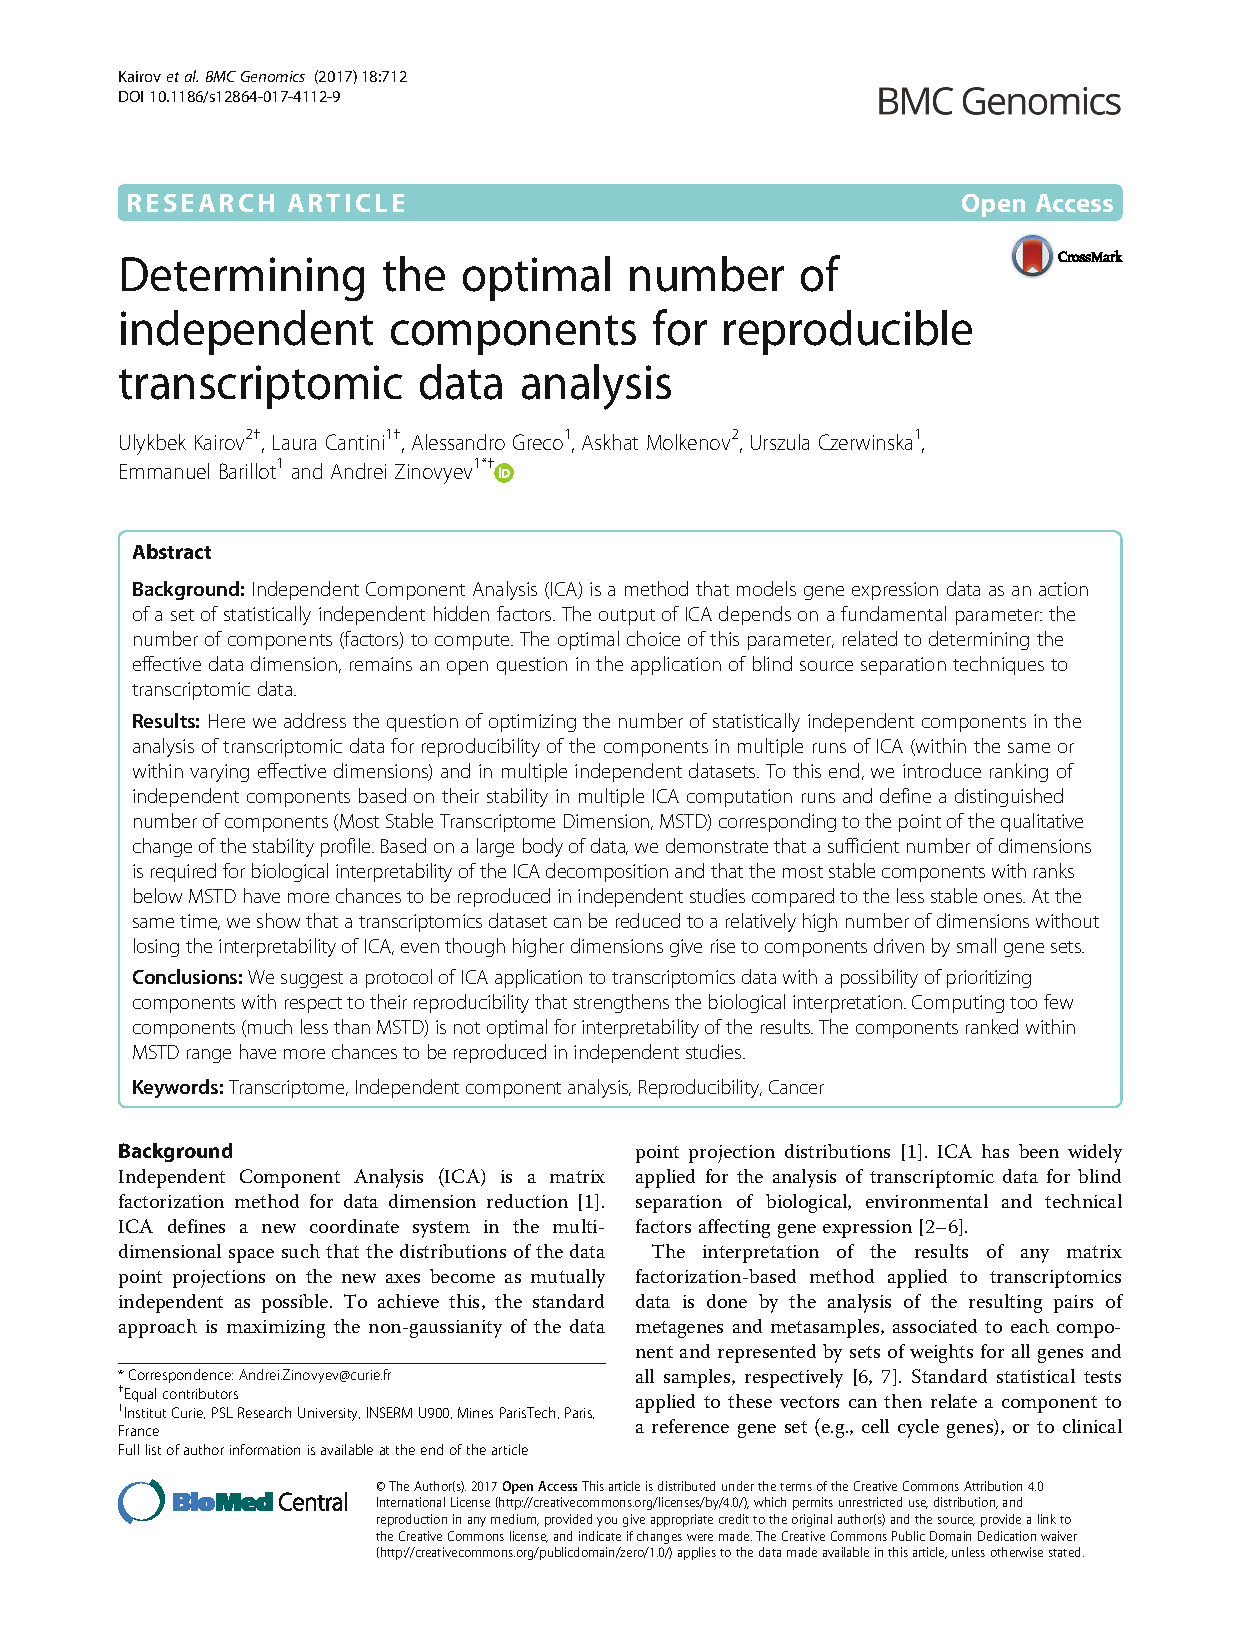
\includepdf[pages={1-}, scale=1]{pdf-ext/BMCMSTD.pdf}

\hypertarget{cell-type-deconvolution-models}{%
\section{Cell-type deconvolution
models}\label{cell-type-deconvolution-models}}

(families of approaches/strategies)

\hypertarget{basis-matrix}{%
\subsection{basis matrix}\label{basis-matrix}}

\begin{itemize}
\tightlist
\item
  define what basis matrix is vs signatures vs marker genes
\item
  explain the differences between basis matrices in published algorithms
\end{itemize}

\hypertarget{regression-algorithm}{%
\subsection{regression algorithm}\label{regression-algorithm}}

\begin{itemize}
\tightlist
\item
  explain what it is for
\item
  explain how it works
\item
  explain the different approaches
\end{itemize}

\hypertarget{others}{%
\subsection{Others}\label{others}}

\begin{itemize}
\tightlist
\item
  explain possible normalisation
\item
  explain additional possible features
\end{itemize}

\hypertarget{short-review-of-most-popular-cell-type-deconvolution-tools}{%
\section{Short review of most popular cell-type deconvolution
tools}\label{short-review-of-most-popular-cell-type-deconvolution-tools}}

Tools will already be mentioned in the section above. However a comment
on other than mentioned aspects are needed.

Explain the success of CIBEROSRT

Explain originality of each tool

\hypertarget{methodological-dimension-of-the-thesis}{%
\section{Methodological dimension of the
thesis}\label{methodological-dimension-of-the-thesis}}

\begin{itemize}
\tightlist
\item
  expose state of art and compare existing tools
\item
  adjustment of existing methodology
\item
  develop a new user-friendly tool
\item
  discuss limitations of computational approaches in biology
\end{itemize}

\hypertarget{sens}{%
\chapter{Study of sensitivity and reproducibility of known
methods}\label{sens}}

\hypertarget{reproducibility-of-nmf-versus-ica-vs-cam}{%
\section{Reproducibility of NMF versus ICA (vs
CAM?)}\label{reproducibility-of-nmf-versus-ica-vs-cam}}

NMF and ICA are both algorithms often applied to solve blind source
deconvolution problem. NMF gained a popularity as a tool of
transcriptomic analysis mainly thanks to the publications
{[}publicaition\_list{]}. However, the non-negativity contraint, an
attractive concept in the case of non-negative transcriptome counts, may
be a reason why the reusults of NMF decomposition are not the best
candidate for our deconvolution task. We observed that NMF-based
metagenes are less reprouctible between different transcriptomic
datasets than ICA-based metagenes.

\hypertarget{comparing-metagenes-obtained-with-nmf-vs-ica.}{%
\subsection{Comparing metagenes obtained with NMF vs
ICA.}\label{comparing-metagenes-obtained-with-nmf-vs-ica.}}

We compared the reproducibility of NMF and ICA through decomposition of
four breast cancer datasets (BRCATCGA, METABRIC, BEK, WAN){[}ref{]}.
Those datasets were selected because of their size (number of samples
\textgreater{} 50) and because they were available in not centred format
necessary for NMF.

For NMF the procedure was following:

\begin{itemize}
\tightlist
\item
  data was transformed into log2
\item
  zero rows were removed
\item
  the algorithm assesing cophentic index was applied to chose optimal
  number of components
\item
  datasets were decomposed with matlab NMF implementation from Brunet et
  al. \citep{Brunet} into (i) number of components suggested by
  cophenetic coefficient (ii) MSTD dimension (iii) 50 components
  (approaching overdecomposition)
\item
  the obtained metagenes were decorellated from the mean using a linear
  regression model
\end{itemize}

For ICA, the procedure was following:

\begin{itemize}
\tightlist
\item
  data were transformed into log2
\item
  transformed data were mean-centered by gene
\item
  our implementation of MSTD (most stable transcriptomic dimension) from
  \citep{Ulykbek2017} was used to evaluate most stable dimension
\item
  datasets were demposed into (i) MSTD dimension and (ii) 50 components
  (approaching overdecomposition) with matlab implementantion of fastICA
  with icasso stabilisation
\end{itemize}

We did not decompose ICA into low number of components as we consider it
as strong underdecomposition and we suspect signals would not be the
most reproducible. We limited the over decomposition higher than 50 with
NMF as for our biggest dataset (METABRIC) NMF decomposition into 50 took
30245 minutes (3 weeks).

Then separately for NMF and ICA, we correlated all obtained metagens
with each other and with known Biton et al.~metagenes (obtain from
previous ICA decompostion applied pan-cancer). We represented the
results in a form of a correlation graph where nodes are metagenes from
different datasets and decompostion levels and edge width corresponds
peasron correaltion coefficients (Fig \ref{fig:ICAvsNMF}).

\begin{figure}

{\centering 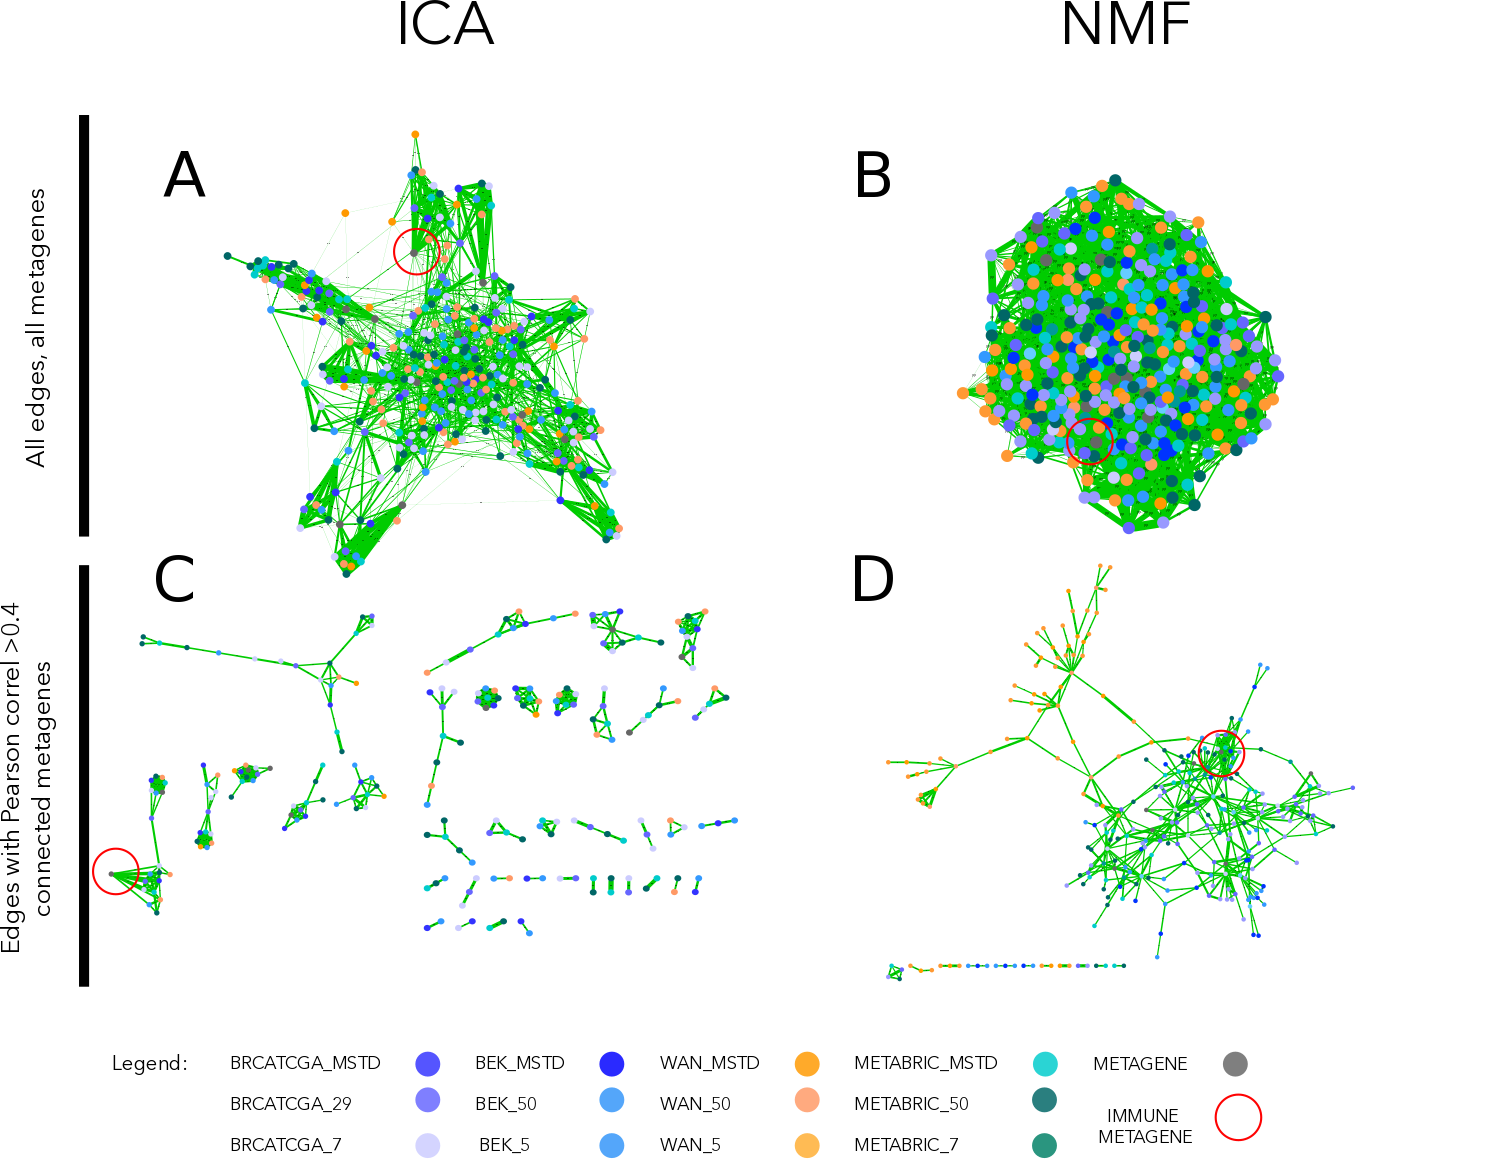
\includegraphics[width=1\linewidth]{figures-ext/ICANMF} 

}

\caption{\textbf{Correlation graph of ICA and NMF multiple
decompositions.} In the upper part of the figure (A,B) we observe the
correlation graph of all metagenes (ICA or NMF-based) disposed using
edge-weighted bio layout. In the lower part of the figure (C,D) we
applied \textgreater{}0.4 thereshold in order to filter the edges. In
the case of ICA (C), remaining nodes form pseudo-cliques, immune-related
pseudo-clique is highlighted. In the case of NMF (D), components cluster
by dataset. Edges' width coressponds to Pearson correlation coefficient.
Node colors correspond to dataset from which a metagene was obtained
(see legend).}\label{fig:ICAvsNMF}
\end{figure}












We hoped to observe a subset of components from different datasets (no
matter the decomposition level) correlate with each strongly and much
less with other components in order to confirm that the signal is
reproducible (can be found in several dataset) and specific. We used the
Biton et al.~componets here to help with eventual identification of
signals (labelling). What we observe from ICA-decomposition that indeed,
without applying any threshold some emerging clusters can be remarked
and after application of \textgreater{}0.4 threshold on the correlation
coeffcient pseudo-cliques emerge. While metagenes from NMF-decpmpostion
are more tighlty connected globally and when the threshold is applied,
remaing metagenes do not form clear clusters but group by data set. In
NMF decomposition if it hard to define different signals as the datasets
seem to be all related to each other. We can see from (Fig
\ref{fig:ICAvsNMF}D) that the IMMUNE signal is correlated
\textgreater{}0.4 with a high number of NMF components that are also
linked to some other components. In ICA (Fig \ref{fig:ICAvsNMF}C)
components related to the IMMUNE metagens form a pseudo-clique that is
related with one link to INTERFERON metagene.

This simple analysis illustrates that NMF applied to cancer
transcriptomes decomposes them to metagenes that are not highly
reproductible between datasets. In practice, it will not always be
possible to work with big cohorts and the same processing methods. Using
ICA for decomposition gives mor credit that it will be possible to use
the obtained metagenes as reference in which new data of similar type
could be projected.

\emph{to do:}

\begin{itemize}
\item
  \emph{quantify: with clustering coefficient?}

  ​
\item
  Explain why ICA is more reproducible
\end{itemize}

\hypertarget{impact-of-modification-of-signatures-list-on-result-for-signature-based-deconvolution-methods}{%
\section{Impact of modification of signatures list on result for
signature-based deconvolution
methods}\label{impact-of-modification-of-signatures-list-on-result-for-signature-based-deconvolution-methods}}

Carry on a ``sensitivity study'':

\begin{itemize}
\tightlist
\item
  remove some \% of genes from basis matrix or marker gene list
\item
  evaluate how it changes results
\end{itemize}

\hypertarget{deconica}{%
\chapter{Deconvolution of transcriptomes and
methylomes}\label{deconica}}

We describe our methods in this chapter. The pre-eliminary pipeline and
simple results are described in the manuscript submitted to
Springer-Verlag's Lecture Notes in Computer Science
(\href{http://www.springer.com/gb/computer-science/lncs}{LNCS}) entitled
\textbf{Application of Independent Component Analysis to Tumor
Transcriptomes Reveals Specific And Reproducible Immune-related Signals}
that is placed at the end of this chapter. In the final thesis final
pipeline will be split into following structure

\hypertarget{from-blind-deconvolution-to-cell-type-quantification-general-overview}{%
\section{From blind deconvolution to cell-type quantification: general
overview}\label{from-blind-deconvolution-to-cell-type-quantification-general-overview}}

Few lines describing our idea

Figure?

\hypertarget{the-ica-based-deconvolution-of-transcriptomes}{%
\subsection{The ICA-based deconvolution of
Transcriptomes}\label{the-ica-based-deconvolution-of-transcriptomes}}

\begin{itemize}
\tightlist
\item
  remind shortly ICA
\item
  describe stabilisation procedure \emph{icasso}
\item
  explain IC-metagene concept
\end{itemize}

If completed add related section about two other ways of getting
metagenes

\begin{itemize}
\tightlist
\item
  attractor metagenes
\item
  k-lines
\end{itemize}

\hypertarget{interpretation-of-independent-components}{%
\subsection{Interpretation of Independent
components}\label{interpretation-of-independent-components}}

\hypertarget{correlation-based-identification-of-confounding-factors}{%
\subsubsection{Correlation based identification of confounding
factors}\label{correlation-based-identification-of-confounding-factors}}

\hypertarget{identification-of-immune-cell-types-with-enrichment-test-other}{%
\subsubsection{Identification of immune cell types with enrichment test
/
other}\label{identification-of-immune-cell-types-with-enrichment-test-other}}

\hypertarget{transforming-metagenes-into-signature-matrix}{%
\subsection{Transforming metagenes into signature
matrix}\label{transforming-metagenes-into-signature-matrix}}

\hypertarget{regression-based-estimation-of-cell-type-proportions-solving-system-of-equations}{%
\subsection{Regression-based estimation of cell-type proportions :
solving system of
equations}\label{regression-based-estimation-of-cell-type-proportions-solving-system-of-equations}}

\hypertarget{deconica-r-package-for-ica-based-deconvolution}{%
\section{\texorpdfstring{\emph{DeconICA} R package for ICA-based
deconvolution}{DeconICA R package for ICA-based deconvolution}}\label{deconica-r-package-for-ica-based-deconvolution}}

This part of the chapter will be adapted from package vignettes

It will contain

\begin{itemize}
\item
  technical package description
\item
  user guide
\item
  examples
\end{itemize}

\hypertarget{demo}{%
\subsection{\texorpdfstring{\emph{Demo}}{Demo}}\label{demo}}

The package needs to installed and then imported.

\begin{Shaded}
\begin{Highlighting}[]
\CommentTok{#import package}
\KeywordTok{library}\NormalTok{(deconica)}
\end{Highlighting}
\end{Shaded}

Then we can perform our pipeline on sample data available in the package

\begin{Shaded}
\begin{Highlighting}[]
\CommentTok{#import sample data}
\KeywordTok{data}\NormalTok{(BRCA)}
\CommentTok{#decompose data}
\NormalTok{fastica.res <-}\StringTok{ }\KeywordTok{run_fastica}\NormalTok{ (}
\NormalTok{  BRCA,}
  \DataTypeTok{optimal =} \OtherTok{TRUE}\NormalTok{,}
  \DataTypeTok{row.center =} \OtherTok{TRUE}\NormalTok{,}
  \DataTypeTok{with.names =} \OtherTok{TRUE}\NormalTok{,}
  \DataTypeTok{gene.names =} \OtherTok{NULL}\NormalTok{,}
  \DataTypeTok{alg.typ =} \StringTok{"parallel"}\NormalTok{,}
  \DataTypeTok{method =} \StringTok{"C"}\NormalTok{,}
  \DataTypeTok{n.comp =} \DecValTok{100}\NormalTok{,}
  \DataTypeTok{isLog =} \OtherTok{TRUE}\NormalTok{,}
  \DataTypeTok{R =} \OtherTok{TRUE}
\NormalTok{)}
\CommentTok{#correlate obtained metagenes with Biton et al. }
\CommentTok{#metagenes (by default)}
\NormalTok{correlate.res <-}
\StringTok{  }\KeywordTok{correlate_metagenes}\NormalTok{(fastica.res}\OperatorTok{$}\NormalTok{S, fastica.res}\OperatorTok{$}\NormalTok{names)}
\CommentTok{#assign reciprocal components}
\NormalTok{assign.res <-}\StringTok{ }\KeywordTok{assign_metagenes}\NormalTok{(correlate.res}\OperatorTok{$}\NormalTok{r)}
\CommentTok{#identify components that are >0.1 correlated with }
\CommentTok{#immune and are not assigned to any other component}
\NormalTok{identify.immune <-}
\StringTok{  }\KeywordTok{identify_immune_ic}\NormalTok{(correlate.res}\OperatorTok{$}\NormalTok{r[, }\StringTok{"M8_IMMUNE"}\NormalTok{], assign.res[, }\DecValTok{2}\NormalTok{])}
\CommentTok{#test enrichment with fisher test in }
\CommentTok{#Immgen signatures (by default)}
\NormalTok{enrichment.res <-}\StringTok{ }\KeywordTok{gene.enrichment.test}\NormalTok{(}
\NormalTok{  fastica.res}\OperatorTok{$}\NormalTok{S,}
\NormalTok{  fastica.res}\OperatorTok{$}\NormalTok{names,}
  \KeywordTok{names}\NormalTok{(identify.immune),}
  \DataTypeTok{gmt =}\NormalTok{ ImmgenHUGO,}
  \DataTypeTok{alternative =} \StringTok{"greater"}\NormalTok{,}
  \DataTypeTok{p.adjust.method =} \StringTok{"BH"}\NormalTok{,}
  \DataTypeTok{p.value.threshold =} \FloatTok{0.05}
\NormalTok{)}
\end{Highlighting}
\end{Shaded}

The present state of the package is described in Fig
\ref{fig:deconICAflow}.

\begin{figure}

{\centering 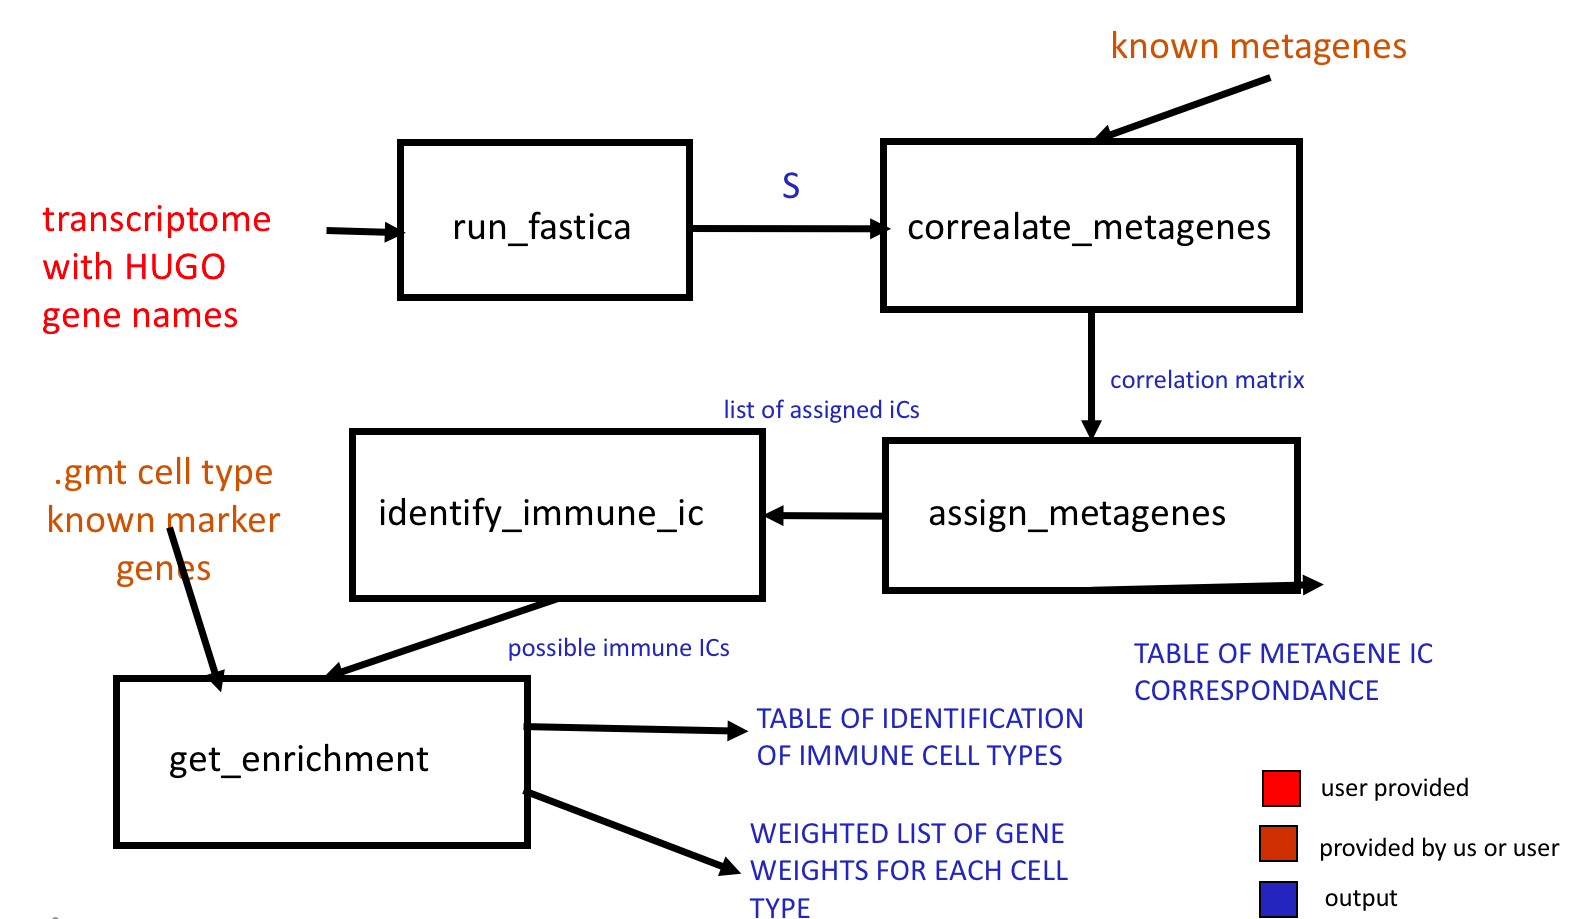
\includegraphics[width=1\linewidth]{figures-ext/deconICApipeline} 

}

\caption{\textbf{State of the deconICA package in
January 2018.} The flow chart illustrates existing functions in the R
package \emph{DeconICA}. Squares represent functions, red are
user-provided inputs, brown are inputs we provide but that can be
replaced easily by user and in blu we marked outputs.}\label{fig:deconICAflow}
\end{figure}







Next step will be:

\begin{itemize}
\tightlist
\item
  adding the metagenes selection and transformation into basis matrix
  for deconvolution
\item
  identifying confounding factors
\item
  estimating purity with an existing tool
\item
  running an equations solver (based on least squares or other type of
  regression) including basis matrix, confounding factors, purity
\item
  including regularisation factos
\item
  adding graphics
\item
  adding user interface
\item
  writing a demo (best interactive)
\end{itemize}

\newpage

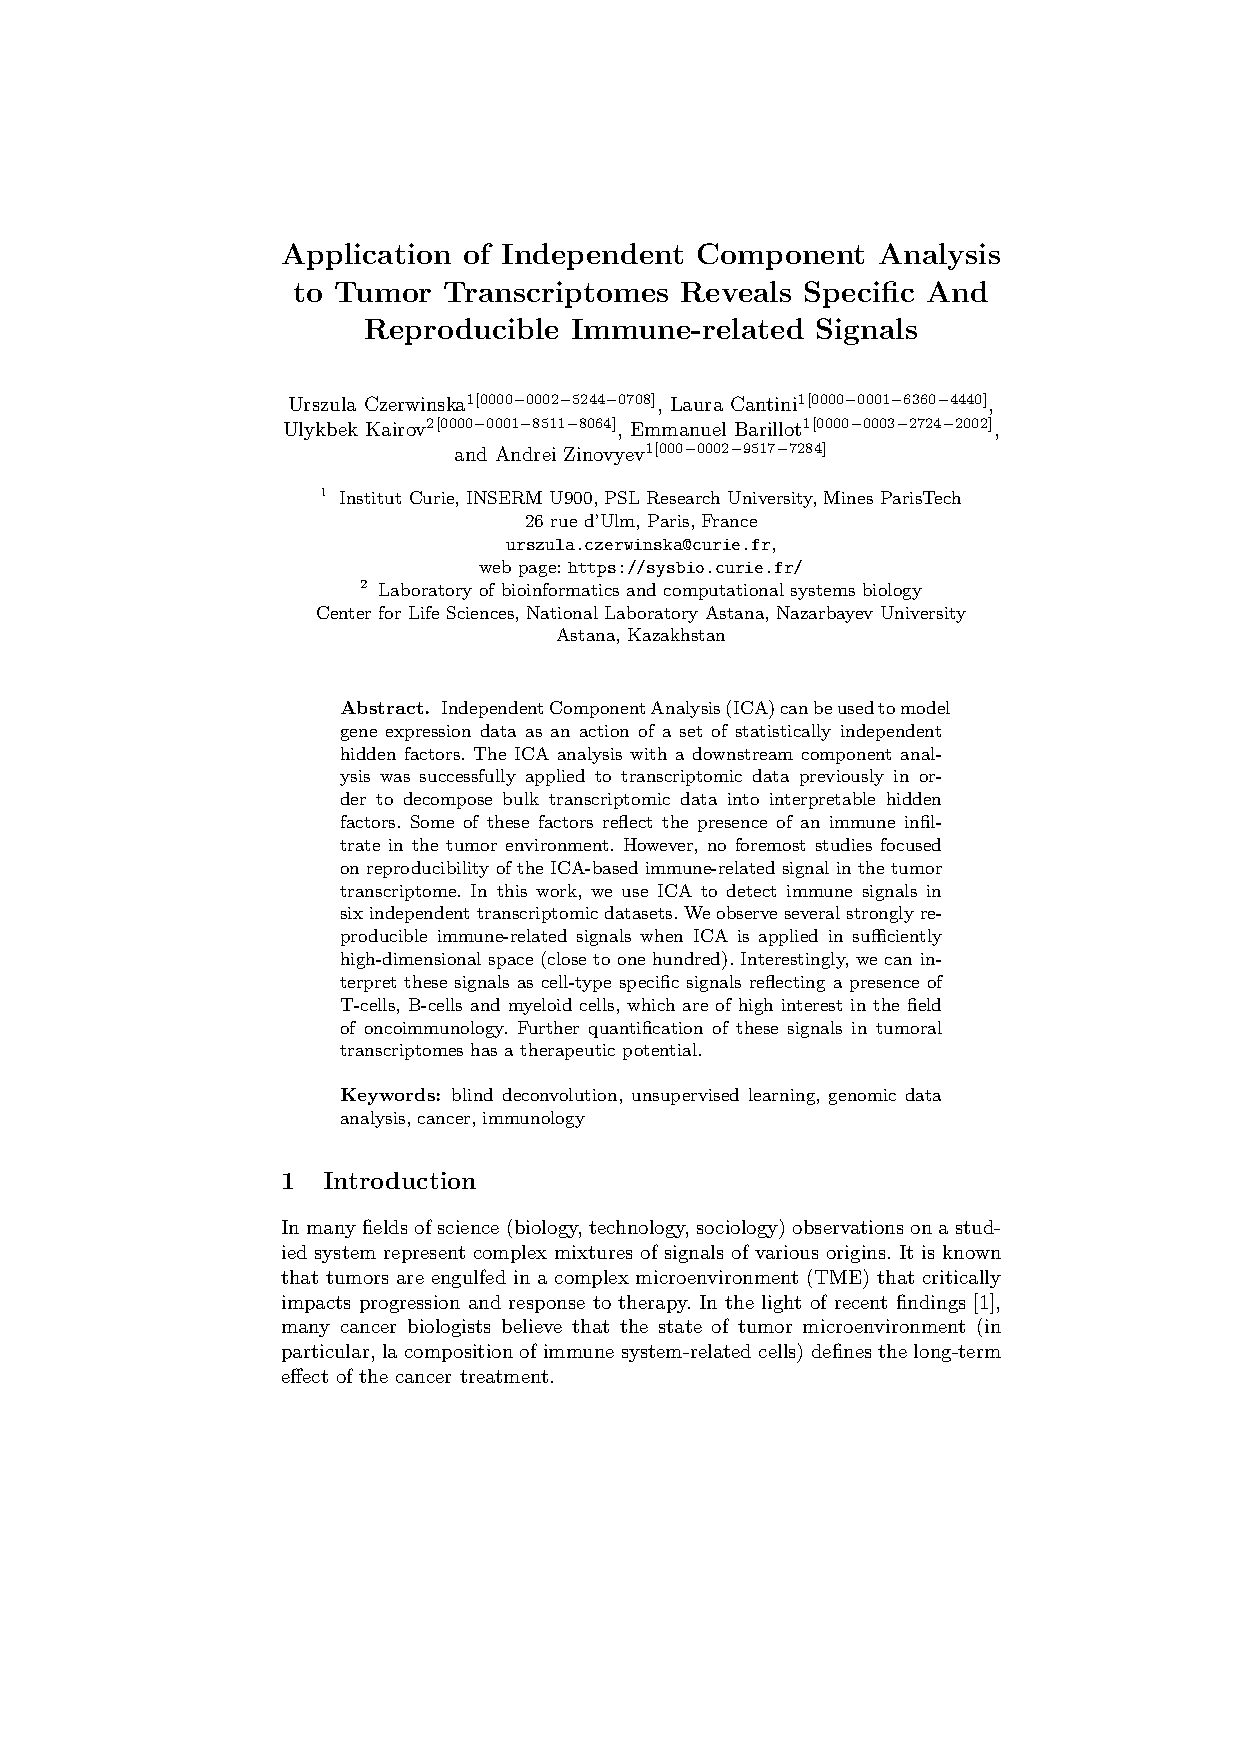
\includepdf[pages={1-}, scale=1]{pdf-ext/LVAICA.pdf}

\hypertarget{results}{%
\chapter{Comparative analysis of cancer immune
infiltration}\label{results}}

This chapter will include biological interpretation of Pan-cancer
analysis with DeconICA

\begin{itemize}
\item
  application to Breast cancer

  \begin{itemize}
  \item
    compare metagenes of the same cell type in different datasets
  \item
    compare metagenes of the same cell type in the same dataset (happens
    sometimes)
  \item
    compare A matrix (sample weights) with clinical metadata
  \item
    compare patients with opposite extreme phenotypes (the gene
    expression) with DEG ou others
  \item
    run enrichment with more specific list of genes ex. Th1/2/17 cells
    in T cels etc.

    ​
  \end{itemize}
\item
  application pan cancer

  \begin{itemize}
  \tightlist
  \item
    derivation of meta-metagenes for immune cell types
  \item
    above points are true for pan cancer
  \end{itemize}
\item
  follow up of Biton paper ?

  \begin{itemize}
  \tightlist
  \item
    \emph{Idea of Vassili from the lab meeting}, personally I am not
    sure if there is no conflict of interest with other members of the
    team
  \end{itemize}
\end{itemize}

\hypertarget{map}{%
\chapter{Heterogeneity of immune cell types}\label{map}}

We include here an extract of a \emph{ready to submit} article of
Kondratova et al. \textbf{(co-first authored by Urszula Czerwinska)} -
the abstract and figures which are result of work on single cell
heterogeneity.

Explication how deconvolution methodology can be used for analysis of
heterogeneity of immune cells

\begin{itemize}
\item
  describe the context briefly
\item
  describe more in details my part - data analysis of single cell data
\end{itemize}

To be defined:

\begin{itemize}
\tightlist
\item
  add CAFS (that will maybe appear in \emph{JBM})
\item
  add unpublished analysis made for the Nature Immunology \emph{Michea
  et al.} paper (to be defined)
\item
  The single T-cell study (if done)
\end{itemize}

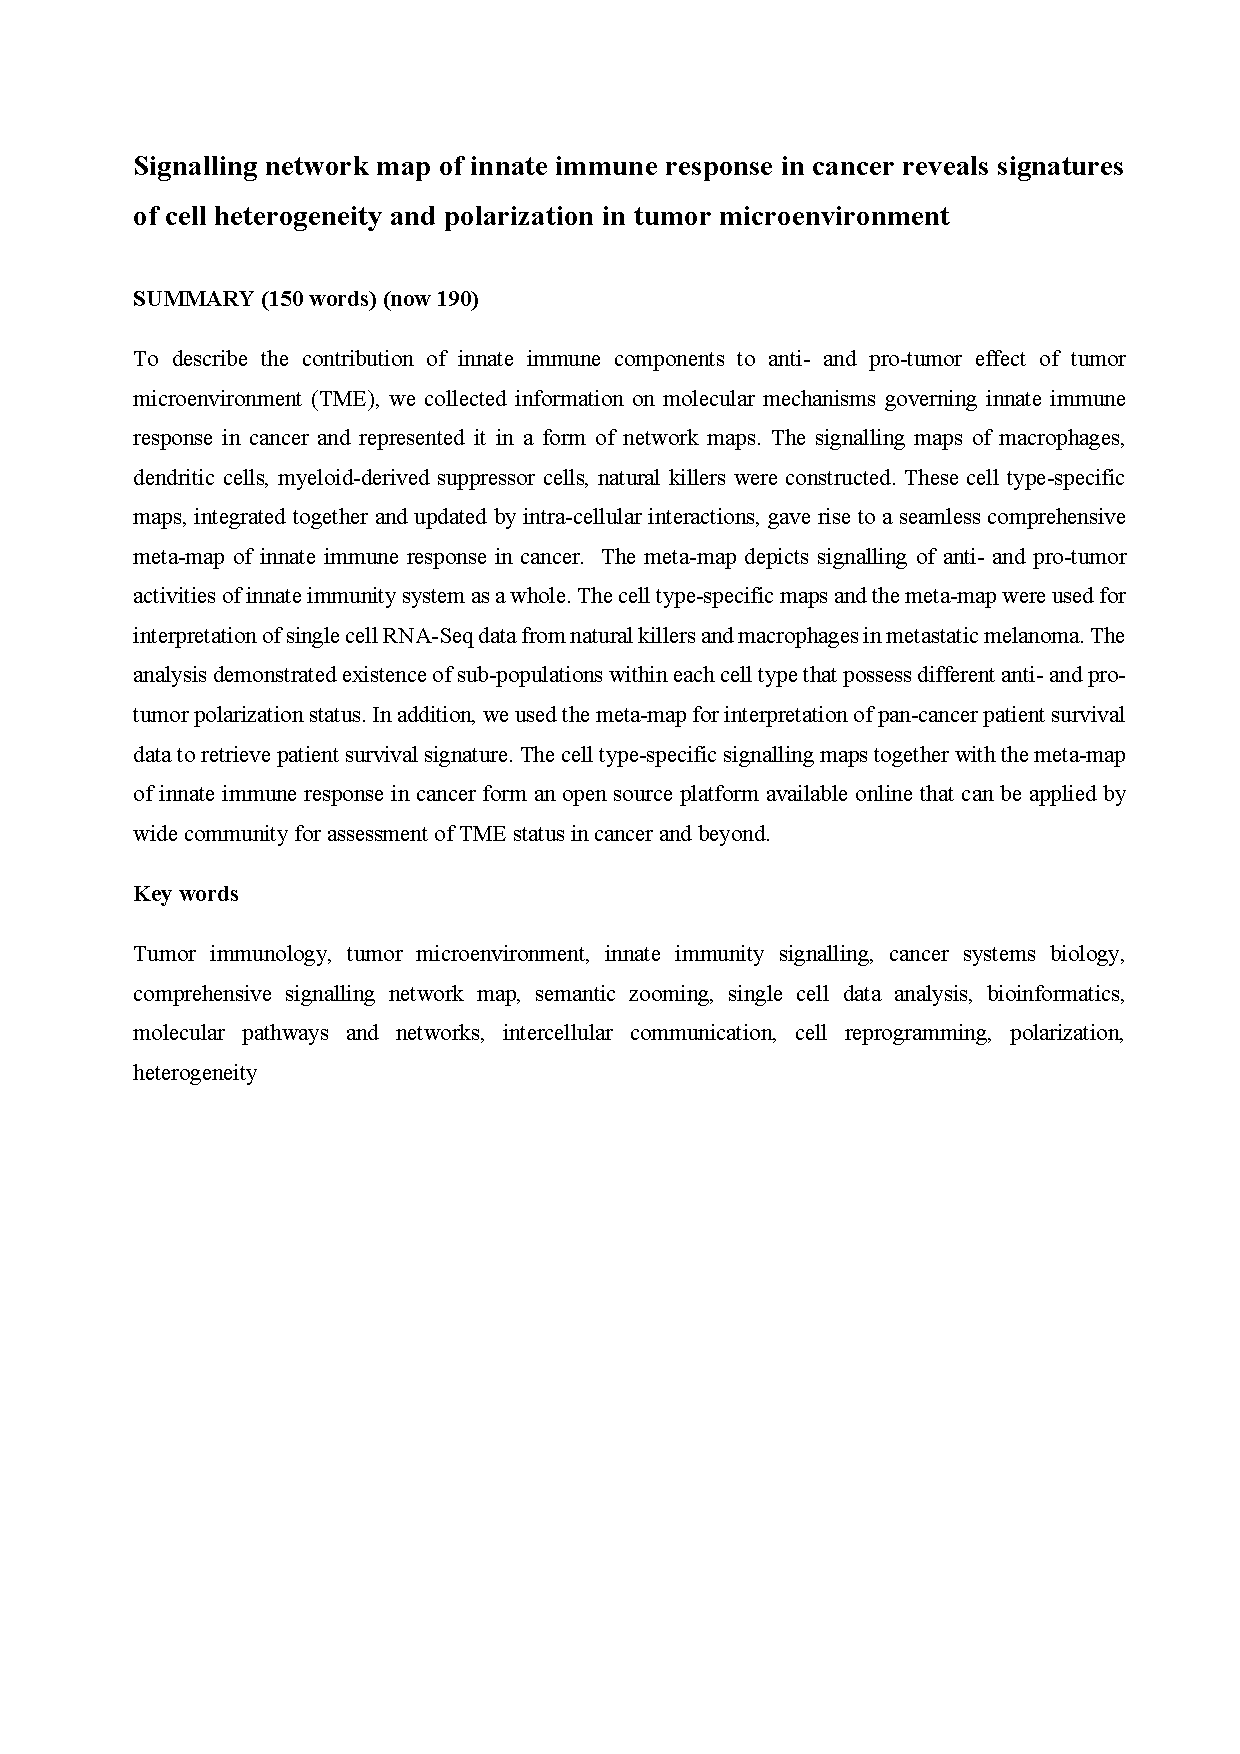
\includepdf[pages={1-}, scale=1]{pdf-ext/ImmuneMap.pdf}

\hypertarget{conclusions}{%
\chapter{Conclusions and perspectives}\label{conclusions}}

Here we will have some interesting and well-written conclusion that will
validate the quality of this thesis.

\hypertarget{annexes}{%
\chapter*{Annexes}\label{annexes}}
\addcontentsline{toc}{chapter}{Annexes}

\emph{Note: This annexe will not be a part of final manuscript}

\hypertarget{phd-timeline-for-defence-before-the-end-of-october-2018}{%
\section*{PhD timeline for defence before the end of October
2018}\label{phd-timeline-for-defence-before-the-end-of-october-2018}}
\addcontentsline{toc}{section}{PhD timeline for defence before the end
of October 2018}

In order to defend before 31 October, I need to follow the guidelines of
the University.

\begin{itemize}
\tightlist
\item
  \textasciitilde{}29 June - officially submlit the jury proposal and a
  draft of the thesis to the university
\item
  \textasciitilde{}end of July - send manuscript to reviewers
\item
  24 Septemeber - 31 October - defend
\end{itemize}

\begin{figure}
\centering
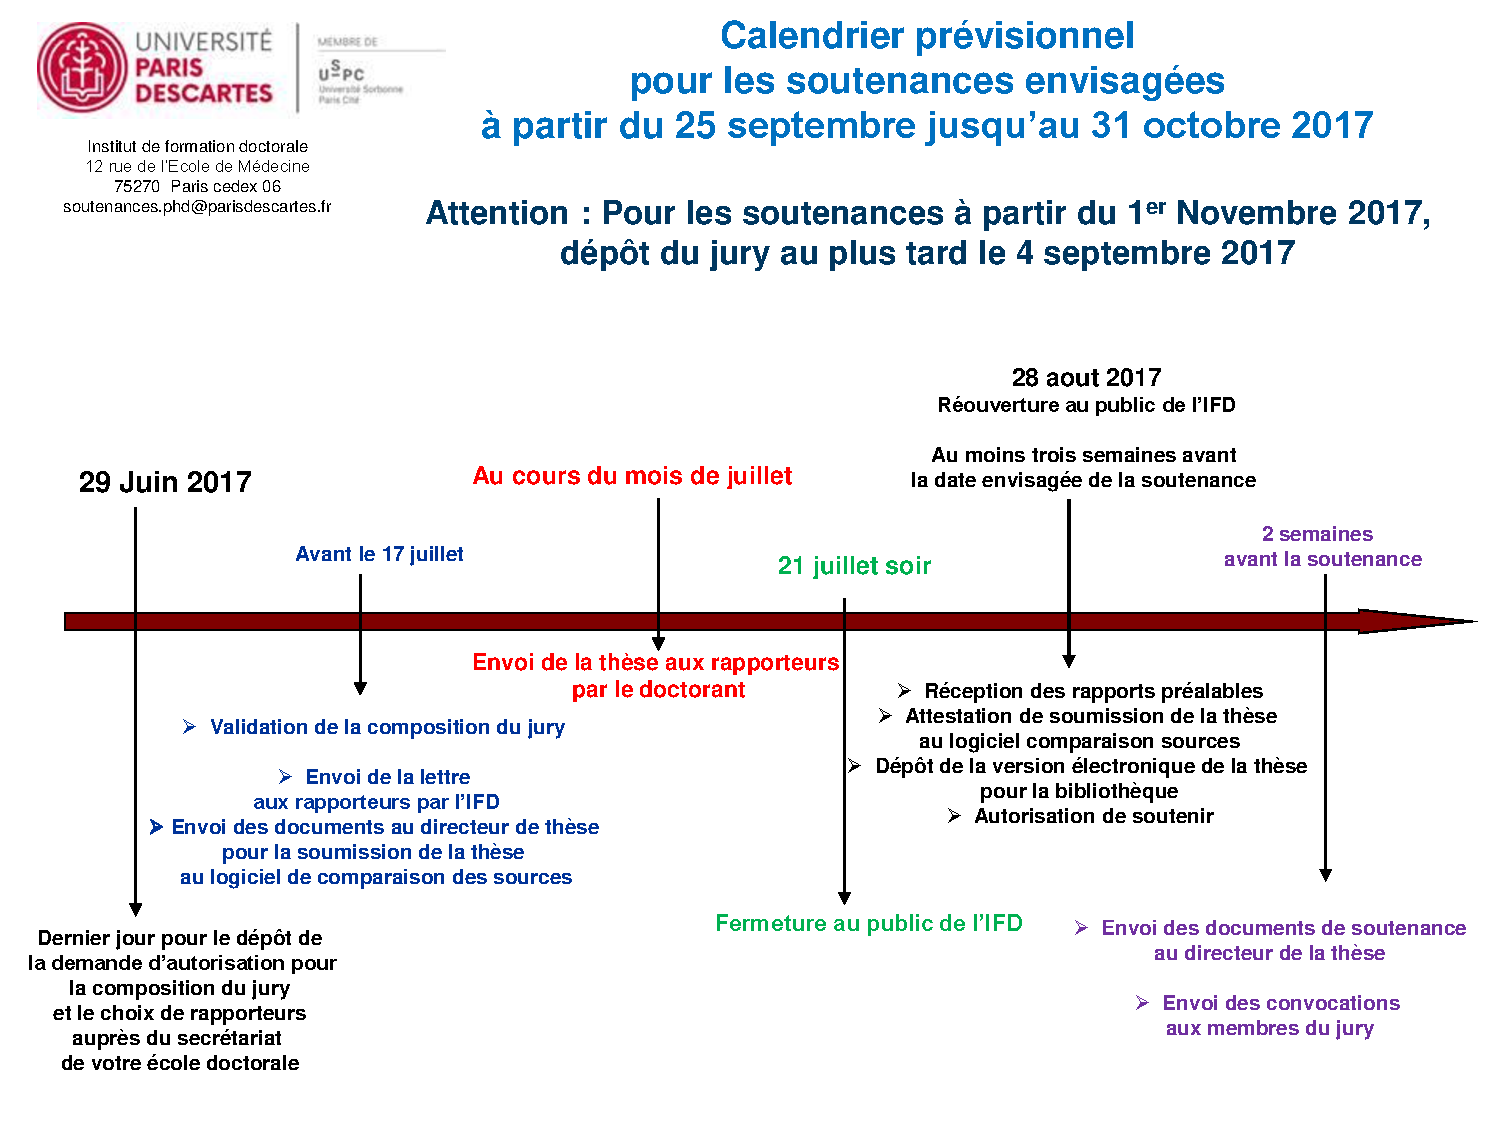
\includegraphics{figures-ext/An-timeline.pdf}
\caption{Timeline provided by University Paris Descartes for 2017}
\end{figure}

\hypertarget{thesis-writing}{%
\section*{Thesis writing}\label{thesis-writing}}
\addcontentsline{toc}{section}{Thesis writing}

This Report is written in
\href{https://github.com/rstudio/bookdown}{\emph{bookdown}}. I have
chosen this form as it can easily compile to \emph{LaTeX}, PDF, MS Word,
ebook and html. Optimally, the final manuscript will be also published
online in a form of an open source
\href{https://www.gitbook.com/about}{gitBook} and an ebook including
interactive figures and maybe even data demos. Another good reason for
using \href{https://github.com/rstudio/bookdown}{\emph{bookdown}} is its
simple syntax of markdown and natural integration of code snippets with
.Rmd. It reduces formatting time and give multiple outputs.

The template of for this thesis manuscript was adapted from \emph{LaTeX}
template provided by University Paris Descartes.

Citations are stocked in Mendeley Desktop and exported to .bib files
automatically.

\href{https://ramblingacademic.com/2016/06/fixing-bibtex-files-mendeley/}{MendeleyBibFix}
is used to cope with automatic export errors.

The format \emph{thesis by publication} will be considered for parts of
the thesis.

\newpage

\hypertarget{activity-report-2017}{%
\section*{Activity Report 2017}\label{activity-report-2017}}
\addcontentsline{toc}{section}{Activity Report 2017}

This documents list main achievements of 2017 including conference,
posters and publications list.

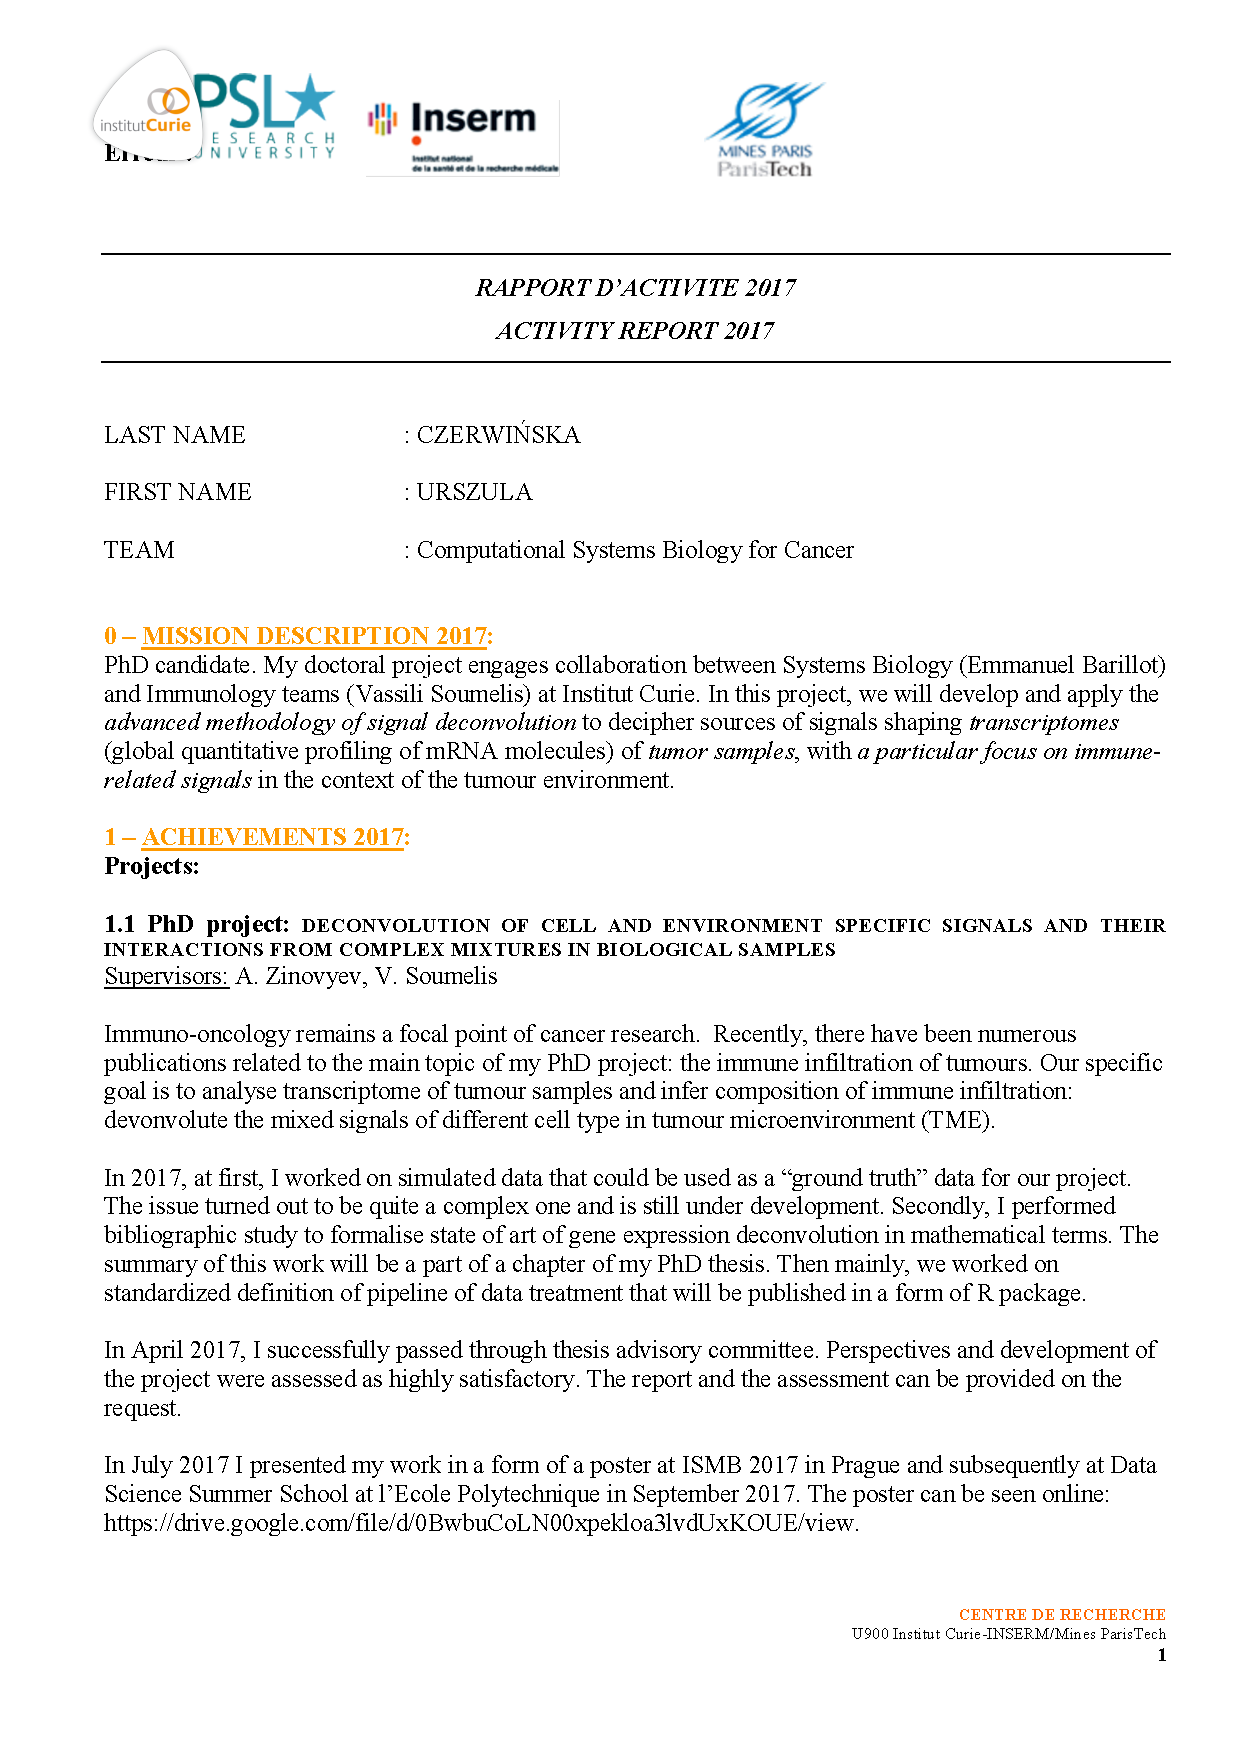
\includepdf[pages={1-}, scale=1]{pdf-ext/An-RA2017.pdf}

\bibliography{00-Inter.bib,01-Intro.bib,packages.bib,UCzcite.bib}


\end{document}
